\documentclass[runningheads]{llncs}
%
\usepackage[T1]{fontenc}
% T1 fonts will be used to generate the final print and online PDFs,
% so please use T1 fonts in your manuscript whenever possible.
%
\usepackage{graphicx}
\usepackage{amsmath, amssymb}
\usepackage{booktabs}
\usepackage{float}
\usepackage{array}
\usepackage{multirow}
\usepackage{enumitem}
\usepackage{algorithm}
\usepackage{algorithmic}
\usepackage{color}
\usepackage{hyperref}
\hypersetup{colorlinks=true, linkcolor=black, citecolor=black, urlcolor=blue}
\renewcommand\UrlFont{\color{blue}\rmfamily}
\urlstyle{rm}

\graphicspath{{report_assets/report_assets/}{experiment_assets/training_curves/}{experiment_assets/confusion_matrices/}}
%
\begin{document}
%
\title{IndoLepAtlas: A Fine-Grained Dataset of Indian Lepidoptera with Geotemporal Metadata and Baseline Classification Study}
%
\titlerunning{IndoLepAtlas: An India--Specific Lepidoptera Dataset}
%
\authorrunning{A. Bansal and K. Chaturvedi}
%
\author{
Akshit Bansal\orcidID{0000-1111-2222-3333} \and
Kriti Chaturvedi\orcidID{0009-0002-0897-5585}
}
%
\institute{\email{23ucs529@lnmiit.ac.in}, \email{23ucs625@lnmiit.ac.in}\\
LNM Institute of Information Technology, Jaipur-302031, Rajasthan
}
%
\maketitle

\begin{abstract}
India is home to an extensive range of insect species but is severely underrepresented in global biodiversity datasets. This creates a significant lack of quality training assests for creating region-specific classification architectures. For species of order Lepidoptera (Butterflies \& Moths), with visually striking features that change with geography and climate, the problem is even more pronounced. To mitigate this, we created the IndoLepAtlas, a curated 60,641-image, 967-species \textbf{India-specific butterfly} dataset with geotemporal metadata, early life-stage documentation (9,804 images), and 703 images of larval host plant species. The dataset is curated from images submitted to a community-driven source, and is verified over multiple stages, ensuring quality and diversity in butterfly species. Our dataset was also cross-referenced against INaturalist, a globally reknowned biodiversity dataset, revealing a significant butterfly species coverage gap, which IndoLepAtlas intends to bridge. Fine-grained classification of butterfly species, often with very subtle inter-species differences or even great intra-species differences, poses a compounding problem. Our research leveraged a unique deep-learning model with Coordinate Attention (CA), Multi-Level Feature Intercation (MLFI) and geotemporal feature integration. We also demonstrate the effectiveness of our model in accurately classifying butterfly species, showcasing improvements over other commonly used architectures.

\keywords{Butterflies, Fine-grained Visual Classification, Lepidoptera, Indian Biodiversity, Geotemporal Fusion, Long-tail Distribution, Coordinate Attention}

\end{abstract}

\section{Introduction}

India's 1,500+ Lepidoptera species represent one of the world's richest butterfly biodiversity hotspots. Accurate butterfly species classification from field photohraphs is crucial for tracking, monitoring, research and conservation planning. This task though, fundamentally differs from standard benchmarks because of a variety of reasons like, discriminative features being spatially precise (eyespot location separates genera), hierarchical distribution across scales (texture bands vs overall wing morphology), large variations within a class, small variations between different classes and uneven sampling (dominant species exceed 500 images while 400 rare species have $<$50 images).

Existing global biodiversity datasets--iNaturalist~\cite{vanhorn2018inaturalist}, GBIF--dilute India-specific subspecies representation. Many Indian endemic and regionally restricted species have fewer than 100 research-grade observations in global repositories, creating a critical data gap for conservation-focused AI systems. Furthermore, no existing butterfly classification dataset integrates geotemporal metadata (biogeographic zone, observation season) or documents larval host plant associations--ecological dimensions that could substantially improve classification accuracy and enable applications beyond species identification, such as early-stage detection and habitat suitability mapping.

Standard CNNs fail on this task due to \textit{spatial information collapse}, \textit{progressive texture loss}, \textit{long-tail imbalance} among other reasons.

We make the following contributions:
\begin{enumerate}[label=(\arabic*)]
    \item \textbf{IndoLepAtlas dataset:} 60,641 butterfly images, 967 species, GPS coordinates, observation dates, 9-zone biogeographic mapping, early life-stage documentation (9,804 images), and 703 host plant images-all centered around Indian Lepidotera species.
    \item \textbf{Systematic baseline establishment:} 11-configuration ablation + 6-model comparison providing reproducible baselines.
    \item \textbf{Geotemporal fusion:} Integration of biogeographic zone and seasonal embeddings into butterfly classification pipeline, achieving 89.38\% Top-1 with 2.1$\times$ fewer parameters than ViT-B/16, and verified via geo-shuffled ablation.
\end{enumerate}

\section{Related Work}
\subsection{Fine-Grained Visual Classification}
Fine-grained visual classification (FGVC) aims to distinguish subordinate categories within a superclass--bird species~\cite{wah2011cub}, dog breeds, car models. Key benchmarks include CUB-200-2011~\cite{wah2011cub} (200 bird species, 11,788 images) and iNaturalist~\cite{vanhorn2018inaturalist} (5,000+ species, 675,000 images). Architecturally, the field has progressed from bilinear pooling through channel attention (SE-Net~\cite{hu2018squeeze}) to multi-level feature fusion (FGBNet~\cite{yuan2025fgbnet}). Vision Transformers~\cite{dosovitski2021image} achieve strong results on large-scale FGVC but require substantial data. Coordinate Attention~\cite{hou2021coordinate} offers a lightweight alternative that preserves spatial structure--a property we exploit for wing-pattern localisation.
\subsection{Insect Classification Datasets and Systems}
The systematic literature review by Amarathunga et al.~\cite{amarathunga2021slr} surveyed insect image classification comprehensively: only 10 of 28 insect orders covered, no Africa or South Asia representation, no morphologically similar microscopic species datasets, and temporal distribution flagged as an explicit open problem. The thrips classification work~\cite{amarathunga2022thrips} is the most relevant morphological similarity study---domain-knowledge-driven body-segment augmentation with ViT achieved 94.7\% on microscopic insects, analogous to our challenges. Alfatemi et al.~\cite{alfatemi2024birds} established methodology for manual data curation in visually similar bird species, a protocol we adapt for Lepidoptera.

\subsection{Geotemporal Context in Species Recognition}
The SLR~\cite{amarathunga2021slr} explicitly identifies temporal and geographic distribution as open problems. Our geotemporal fusion module directly addresses this gap. In addition to geotemporal context, the dataset also provides images of larval stages and larval host plants for further classification enhancements or behaviour modelling.

\begin{figure}[H]
\centering
% Row 1: Kallima pair + Rose pair
\begin{minipage}{0.24\linewidth}\centering
    \includegraphics[width=\linewidth,height=3.2cm,keepaspectratio]{report_assets/butterfly_comp/geo_comp/Kalilima_inachus_himalayas.jpg}\\
    {\scriptsize (a) \textit{Kallima inachus}\\Himalayas}
\end{minipage}\hfill
\begin{minipage}{0.24\linewidth}\centering
    \includegraphics[width=\linewidth,height=3.2cm,keepaspectratio]{report_assets/butterfly_comp/geo_comp/kallima_horsfieldii_westerghats.jpg}\\
    {\scriptsize (b) \textit{Kallima horsfieldii}\\W. Ghats}
\end{minipage}\hfill
\begin{minipage}{0.24\linewidth}\centering
    \includegraphics[width=\linewidth,height=3.2cm,keepaspectratio]{report_assets/butterfly_comp/geo_comp/common_rose_north.jpg}\\
    {\scriptsize (c) \textit{Pachliopta aristolochiae}\\Himalayas}
\end{minipage}\hfill
\begin{minipage}{0.24\linewidth}\centering
    \includegraphics[width=\linewidth,height=3.2cm,keepaspectratio]{report_assets/butterfly_comp/geo_comp/malabar_rose_south_endemic.jpg}\\
    {\scriptsize (d) \textit{Pachliopta pandiyana}\\W. Ghats}
\end{minipage}

\vspace{0.5em}

% Row 2: Mycalesis pair + Eurema pair
\begin{minipage}{0.24\linewidth}\centering
    \includegraphics[width=\linewidth,height=3.2cm,keepaspectratio]{report_assets/butterfly_comp/geo_comp/Mycalesis_francisca_perdiccas_north.JPG}\\
    {\scriptsize (e) \textit{Mycalesis francisca}\\NE India}
\end{minipage}\hfill
\begin{minipage}{0.24\linewidth}\centering
    \includegraphics[width=\linewidth,height=3.2cm,keepaspectratio]{report_assets/butterfly_comp/geo_comp/mycalesis_gotama_south.jpg}\\
    {\scriptsize (f) \textit{Mycalesis gotama}\\W. Ghats}
\end{minipage}\hfill
\begin{minipage}{0.24\linewidth}\centering
    \includegraphics[width=\linewidth,height=3.2cm,keepaspectratio]{report_assets/butterfly_comp/geo_comp/eurema_brigitta_north.JPG}\\
    {\scriptsize (g) \textit{Eurema brigitta}\\Himalayas}
\end{minipage}\hfill
\begin{minipage}{0.24\linewidth}\centering
    \includegraphics[width=\linewidth,height=3.2cm,keepaspectratio]{report_assets/butterfly_comp/geo_comp/eurema_nilgirensis_south.jpeg}\\
    {\scriptsize (h) \textit{Eurema nilgiriensis}\\Nilgiris}
\end{minipage}
\caption{Four visually near-identical species pairs separated by biogeographic zone. \textbf{(a--b)} \textit{Kallima} dead-leaf butterflies: Himalayas vs.\ Western Ghats. \textbf{(c--d)} Swallowtail roses: widespread Common Rose vs.\ Western Ghats--endemic Malabar Rose. \textbf{(e--f)} \textit{Mycalesis} bush browns: Northeast India vs.\ Western Ghats. \textbf{(g--h)} \textit{Eurema} grass yellows: widespread \textit{E. brigitta} vs.\ Nilgiri--endemic \textit{E. nilgiriensis}. Geographic metadata disambiguates these pairs where visual features alone cannot.} \label{fig:geo_comp}
\end{figure}

\section{IndoLepAtlas Dataset}
The dataset is available at \href{https://huggingface.co/datasets/Butterfree/IndoLepAtlas}{IndoLepAtlas (Hugging Face)}
\begin{figure}[H]
\centering
% Row 1: Monkey Puzzle (Rathinda amor) — Adult, Larva, Egg, Host Plant
\begin{minipage}{0.31\linewidth}\centering
    \includegraphics[width=\linewidth,height=3cm,keepaspectratio]{report_assets/butterfly_comp/moneky_puzzle.jpg}\\
    {\scriptsize (a) \textit{Monkey Puzzle (Adult)}}
\end{minipage}\hfill
\begin{minipage}{0.31\linewidth}\centering
    \includegraphics[width=\linewidth,height=3cm,keepaspectratio]{report_assets/butterfly_comp/monkey_puzzle_egg.jpg}\\
    {\scriptsize (b) \textit{Monkey Puzzle (Egg)}}
\end{minipage}\hfill
\begin{minipage}{0.31\linewidth}\centering
    \includegraphics[width=\linewidth,height=3cm,keepaspectratio]{report_assets/butterfly_comp/malabar_tree_nymph.jpg}\\
    {\scriptsize (c) \textit{Malabar Tree Nymph (Adult)}}
\end{minipage}\hfill

\vspace{0.2em}
\begin{minipage}{0.31\linewidth}\centering
    \includegraphics[width=\linewidth,height=3cm,keepaspectratio]{report_assets/butterfly_comp/malabar_tree_nymph_larva.jpg}\\
    {\scriptsize (d) \textit{Malabar Tree Nymph (Larva)}}
\end{minipage}\hfill
\begin{minipage}{0.31\linewidth}\centering
    \includegraphics[width=\linewidth,height=3cm,keepaspectratio]{report_assets/butterfly_comp/common_map.jpg}\\
    {\scriptsize (e) \textit{Common Map (Adult)}}
\end{minipage}\hfill
\begin{minipage}{0.31\linewidth}\centering
    \includegraphics[width=\linewidth,height=3cm,keepaspectratio]{report_assets/butterfly_comp/common_map_coccoon.jpg}\\
    {\scriptsize (f) \textit{Common Map (Chrysalis)}}
\end{minipage}\hfill

\vspace{0.2em}
\begin{minipage}{0.31\linewidth}\centering
    \includegraphics[width=\linewidth,height=3cm,keepaspectratio]{report_assets/butterfly_comp/psyche_host.jpg}\\
    {\scriptsize (g) \textit{Psyche (Host plant)}}
\end{minipage}\hfill
\begin{minipage}{0.31\linewidth}\centering
    \includegraphics[width=\linewidth,height=3cm,keepaspectratio]{report_assets/butterfly_comp/psyche.jpg}\\
    {\scriptsize (h) \textit{Psyche (Adult)}}
\end{minipage}\hfill
\begin{minipage}{0.31\linewidth}\centering
    \includegraphics[width=\linewidth,height=3cm,keepaspectratio]{report_assets/butterfly_comp/psyche_egg.jpg}\\
    {\scriptsize (i) \textit{Psyche (Egg)}}
\end{minipage}\hfill
\vspace{0.2em}
% \begin{minipage}{0.24\linewidth}\centering
%     \includegraphics[width=\linewidth,height=3cm,keepaspectratio]{report_assets/butterfly_comp/psyche.jpg}\\
%     {\scriptsize (j) \textit{Leptosia nina}\\Adult}
% \end{minipage}\hfill
% \begin{minipage}{0.24\linewidth}\centering
%     \includegraphics[width=\linewidth,height=3cm,keepaspectratio]{report_assets/butterfly_comp/psyche_egg.jpg}\\
%     {\scriptsize (k) \textit{L. nina}\\Egg}
% \end{minipage}\hfill
% \begin{minipage}{0.24\linewidth}\centering
%     \includegraphics[width=\linewidth,height=3cm,keepaspectratio]{report_assets/butterfly_comp/psyche_host.jpg}\\
%     {\scriptsize (l) \textit{Crateva religiosa}\\Host plant}
% \end{minipage}
\caption{Multi-stage coverage in IndoLepAtlas across four species. \textbf{\textit{Rathinda amor} (Monkey Puzzle)}: adult, egg; \textbf{\textit{Idea malabarica} (Malabar Tree Nymph)}: adult, larva; \textbf{\textit{Leptosia Nina} (Common Psyche)}: adult, egg, host plant. \label{fig4}}
\end{figure}

\subsection{Collection and Curation}
IndoLepAtlas comprises 61,344 images (60,641 butterflies across 967 species + 703 plant images across 127 larval host plant species), curated primarily from the \href{https://www.IFoundButterflies.org}{Indian Lepidoptera web atlas}. The full collection and preparation pipeline is formalised in Algorithm~\ref{alg:curation}.

\begin{algorithm}[H]
\caption{IndoLepAtlas Dataset Collection and Preparation Pipeline}\label{alg:curation}
\begin{algorithmic}[1]
\REQUIRE Raw species galleries $\mathcal{G}$ from IFoundButterflies.org \hfill $\triangleright$ Web source
% \ENSURE Curated dataset $\mathcal{D}$ with images, labels, metadata, and train/val/test splits
\STATE Download all images and metadata pages per species gallery
\STATE Assign class labels
\STATE Extract per-image metadata via OCR
\STATE Remove non-butterfly entries; resolve taxonomic synonyms
\STATE Separate early life-stage images from adult specimens
\STATE Map GPS coordinates to biogeographic zones 
\STATE Encode observation month cyclically
\STATE Assign learned ``unknown'' embedding where GPS or date is missing
\STATE Perform stratified train/val/test split
\STATE Ensure every species appears in all three splits
\RETURN $\mathcal{D}_{\text{train}},\; \mathcal{D}_{\text{val}},\; \mathcal{D}_{\text{test}},\; \mathcal{D}_{\text{early}}$
\end{algorithmic}
\end{algorithm}

\subsection{Statistics}
\begin{table}[H]
    \centering
    \begin{minipage}{0.48\linewidth}
        \centering
        \caption{Family distribution (butterflies)}
        \label{tab:family_distribution}
        \begin{tabular}{|l|l|l|}
            \toprule
            Family & Images & Percentage \\
            \midrule
            Nymphalidae & 18,054 & 29.8\% \\
            Lycaenidae & 16,985 & 28.0\% \\
            Hesperiidae & 12,361 & 20.4\% \\
            Pieridae & 6,132 & 10.1\% \\
            Papilionidae & 5,826 & 9.6\% \\
            Riodinidae & 1,132 & 1.9\% \\
            \bottomrule
        \end{tabular}
    \end{minipage}\hfill
    \begin{minipage}{0.48\linewidth}
        \centering
        \caption{Data splits}
        \label{tab:data_splits}
        \begin{tabular}{|l|l|l|}
            \toprule
            Split & Images & Percentage \\
            \midrule
            Train & 48,630 & 79.3\% \\
            Validation & 5,649 & 9.2\% \\
            Test & 7,065 & 11.5\% \\
            \bottomrule
        \end{tabular}
    \end{minipage}
\end{table}

\subsection{Metadata Description}
\textbf{Location $\rightarrow$ Biogeographic zone:} GPS coordinates mapped to India's 9 established biogeographic zones (Wildlife Institute of India classification): Western Ghats, Deccan Peninsula, Western Himalayas, Eastern Himalayas, Northeast India, Indo-Gangetic Plain, Semi-Arid, Desert, and Andaman \& Nicobar Islands. A 10th "unknown" index is used when GPS is missing. Zone-level encoding is ecologically motivated and robust to typical $\pm$km GPS errors. Each zone is represented as a learned 32-dimensional embedding vector.
Images lacking location or date (cyclically encoded) use a learned "unknown" embedding token during geotemporal fusion.

\subsection{Dataset Quality Validation}
For automated bbox verification, 100 random images per subset are spot-checked and failures are then re-annotated via CVAT. To maintain taxonomic consistency, species labels are inherited from expert-curated \href{https://www.ifoundbutterflies.org}{IFoundButterflies} directory structure, cross-referenced against Indian butterfly field guides~\cite{kehimkar2016butterflies}. Geographic/seasonal distributions are cross-referenced against known species ranges, the confusion matrix analysis (Section~6) confirms systematic confusion occurs between congeneric species.

\subsection{Coverage Gap Analysis}
\begin{table}[H]
\centering
\caption{Comparison with Existing Datasets}
\label{tab:dataset_comparison}
\small
\begin{tabular}{|l|l|l|l|l|l|l|l|}
    \toprule
        \textbf{Dataset} & \textbf{Species} & \textbf{Images} & \textbf{Domain} & \textbf{Location} & \textbf{Temporal} & \textbf{Host Plants} & \textbf{India--specific} \\
    \midrule
        CUB-200-2011 & 200 & 11,788 & Birds & $\times$ & $\times$ & $\times$ & $\times$ \\
        iNaturalist & 5,089 & 675,170 & Multi & $\checkmark$ & $\checkmark$ & $\times$ & $\times$ \\
        IP102~\cite{wu2019ip102} & 102 & 75,222 & Insects & $\times$ & $\times$ & $\times$ & $\times$ \\
        \textbf{IndoLepAtlas} & \textbf{967} & \textbf{60,641} & \textbf{Butterflies} & $\checkmark$ & $\checkmark$ & $\checkmark$ & $\checkmark$ \\
    \bottomrule
    \end{tabular}
\end{table}
\begin{table}
\centering
    \caption{INat Coverage Gap Analysis}
    \label{tab:inat_coverage}
    % \small
    \begin{tabular}{|l|l|l|}
        \toprule
        iNat India Records & \# of Species & \% of Dataset \\
        \midrule
        0 (absent) & 145 & 15.1\% \\
        1–10 & 249 & 25.9\% \\
        11–50 & 194 & 20.2\% \\
        51–100 & 78 & 8.1\% \\
        101–500 & 147 & 15.3\% \\
        $>$500 & 148 & 15.4\% \\
        \bottomrule
    \end{tabular}
\end{table}
% \begin{table}
%     \centering
%     \caption{INat Coverage Gap Analysis}
%     \label{tab:inat_coverage}
%     \small
%     \begin{tabular}{|l|l|l|}
%         \toprule
%         iNat India Records & \# of Species & \% of Dataset \\
%         \midrule
%         0 (absent) & 145 & 15.1\% \\
%         1–10 & 249 & 25.9\% \\
%         11–50 & 194 & 20.2\% \\
%         51–100 & 78 & 8.1\% \\
%         101–500 & 147 & 15.3\% \\
%         $>$500 & 148 & 15.4\% \\
%         \bottomrule
%     \end{tabular}
% \end{table}

Cross-referencing IndoLepAtlas species against iNaturalist India research-grade observations reveals that 69.3\% of our species have fewer than 100 India-specific iNat records, and 145 species (15.1\%) have zero records, confirming the under-representation of Indian Lepidoptera species within global repositories. 

\section{Experimental Setup}
Experiments execute on a DGX V100 cluster in two phases.
\begin{itemize}
    \item \textbf{Backbone:} ConvNeXt-Tiny (ImageNet pretrained)
    \item \textbf{Optimiser:} AdamW, differential learning rates (backbone 0.1$\times$, new heads 10$^{-4}$)
    \item \textbf{Scheduler:} Cosine annealing with 5-epoch warmup
    \item \textbf{Training:} Mixed precision (AMP), gradient norm clipping at 5.0
    \item \textbf{Checkpoint selection:} Best macro-F1 on validation (ensures long-tail sensitivity)
    \item \textbf{Augmentation (train):} Random resized crop, flipping, rotation, color jitter, ImageNet normalisation.
    \item \textbf{Augmentation (val/test):} Deterministic resize + centre crop, ImageNet normalisation.
    \begin{itemize}
        \item Unit I (Loss dynamics): 30 epochs, 4 configs
        \item Units II–III (Architecture, Freezing): 40 epochs, 7 configs
    \end{itemize}
\end{itemize}


\section{Baseline Experiments and Results}

\subsection{Unit I: Long-Tail Loss Dynamics (30 epochs)}

\textbf{Question:} How do different loss formulations and sampling strategies impact representational capacity on long-tailed fine-grained distributions?

\begin{table}
    \centering
    \caption{Validation accuracy for loss--sampling configurations.}
    \begin{tabular}{|l|l|l|l|l|}
        \toprule
    \textbf{Configuration} & \textbf{Top-1 (\%)} & \textbf{Macro F1 (\%)} & \textbf{Dense Acc (\%)} & \textbf{Sparse Acc (\%)} \\
    \midrule
    \textbf{CE + Balanced} & 87.06 & \textbf{85.48} & 87.67 & 85.84 \\
    \textbf{CE + Unbalanced} & \textbf{87.60} & 80.23 & \textbf{91.22} & 80.35 \\
    \textbf{Focal + Balanced} & 82.69 & 82.64 & 80.85 & \textbf{86.40} \\
    \textbf{Focal + Unbalanced} & 84.83 & 82.70 & 85.70 & 83.07 \\
    \bottomrule
    \end{tabular}
    \label{tab:unit1_loss}
\end{table}

\begin{figure}
    \centering
    \begin{minipage}{0.48\linewidth}
        \centering
        \includegraphics[width=\linewidth]{report_assets/report_assets/plots/unit1_training_curves.png}
        \caption{Unit I training curves.} \label{fig5}
    \end{minipage}\hfill
    \begin{minipage}{0.48\linewidth}
        \centering
        \includegraphics[width=\linewidth]{report_assets/report_assets/plots/unit1_bar_comparison.png}
        \caption{Unit I metric comparison.} \label{fig6}
    \end{minipage}
\end{figure}

The model abandons rare species to maximise majority-class performance. Instead, inverse-frequency sampling ensures rare-class gradients remain proportional regardless of distribution skew. Explicit sampling works better for the long-tail problem than loss-function.

\subsection{Unit II: Feature-Fusion Ablation (40 epochs)}

\textbf{Question:} Where is the optimal structural transition point for integrating attention mechanisms, and does multi-level feature integration improve fine-grained classification?

\begin{table}
    \centering
    \caption{Validation accuracy for architectural configurations}
\begin{tabular}{|l|l|l|l|l|}
\toprule
\textbf{Configuration} & \textbf{Top-1 (\%)} & \textbf{Macro F1 (\%)} & \textbf{Dense Acc (\%)} & \textbf{Sparse Acc (\%)} \\
\midrule
\textbf{Phase 1 (Baseline)} & 86.50 & 85.65 & \textbf{86.36} & 86.76 \\
\textbf{+ CA} & \textbf{86.77} & \textbf{85.75} & 86.13 & \textbf{88.05} \\
\textbf{+ CA + MLFI} & 84.43 & 83.34 & 83.32 & 86.66 \\
\bottomrule
\end{tabular}
\label{tab:unit2_loss}
\end{table}

\begin{figure}
    \centering
    \begin{minipage}{0.48\linewidth}
        \centering
        \includegraphics[width=\linewidth]{report_assets/report_assets/plots/unit2_training_curves.png}
        \caption{Unit II training curves.} \label{fig7}
    \end{minipage}\hfill
    \begin{minipage}{0.48\linewidth}
        \centering
        \includegraphics[width=\linewidth]{report_assets/report_assets/plots/unit2_bar_comparison.png}
        \caption{Unit II metric comparison.} \label{fig8}
    \end{minipage}
\end{figure}
Coordinate Attention (CA) preserves spatial morphology. It decomposes channel-spatial attention into two horizontal and vertical pooling — preserving directional structure naturally suited to butterfly morphology (horizontal banding, vertical vein streaking). Unlike SE-Net's global average pooling, CA retains \textit{where} a pattern occurs.
At 40 epochs, MLFI reaches 84.43\% Top-1 and 86.66\% Sparse--demonstrating multi-level fusion does benefit rare classes. The newly initialised MLFI layers (Xavier init, full learning rate) create an optimisation imbalance with the near-converged backbone (0.1$\times$ learning rate), resulting in a poorly conditioned loss landscape.

\subsection{Unit III: Transfer Learning Layer Freezing (40 Epochs)}

\textbf{Question:} Which hierarchical layers contain domain-agnostic vs domain-specific representations, and what is the optimal adaptation pathway?

\begin{table}
    \centering
\caption{Layer Freezing accuracy}
\begin{tabular}{|l|l|l|l|l|}
\hline
\textbf{Configuration} & \textbf{Top-1 (\%)} & \textbf{Macro F1 (\%)} & \textbf{Dense Acc (\%)} & \textbf{Sparse Acc (\%)} \\
\hline
\textbf{End-to-End} & \textbf{84.79} & \textbf{84.11} & \textbf{83.89} & 86.61 \\
\textbf{Head Only} & 53.20 & 57.02 & 44.46 & 70.75 \\
\textbf{Freeze Early} & 83.77 & 83.20 & 82.74 & 85.84 \\
Freeze Late & 84.33 & 84.02 & 83.15 & \textbf{86.71} \\
\bottomrule
\end{tabular}
\label{tab:unit3_transfer}
\end{table}

\begin{figure}
    \centering
    \begin{minipage}{0.48\linewidth}
        \centering
        \includegraphics[width=\linewidth]{report_assets/report_assets/plots/unit3_training_curves.png}
        \caption{Unit III training curves.} \label{fig9}
    \end{minipage}\hfill
    \begin{minipage}{0.48\linewidth}
        \centering
        \includegraphics[width=\linewidth]{report_assets/report_assets/plots/unit3_bar_comparison.png}
        \caption{Unit III metric comparison.} \label{fig10}
    \end{minipage}
\end{figure}
ImageNet activations encode "furry surface textures" and "rounded shapes," not "submarginal band" or "discal spot." Fine-grained biological classification is fundamentally a \textit{domain-shift problem disguised as a classification problem}.
Freezing late blocks (84.33\%) slightly outperforms freezing early blocks (83.77\%), implying early-layer Gabor-like edge detectors require significant recalibration for butterfly wing scales and biological venation. We also observe that full gradient backpropagation achieves the best macro-F1 (84.11\%) and most balanced stratum performance (Dense 83.89\%, Sparse 86.61\%).

\section{Model Comparison}

To contextualise our ablation findings and evaluate our geotemporal fusion module, we benchmark six architectures on the same dataset split (Table~\ref{tab:model_comparison}).
\subsection{Main Comparison}
\begin{table}[H]
\centering
\caption{Model comparison on the test set (40 epochs, CE loss, balanced sampling).}
\label{tab:model_comparison}
\small
\begin{tabular}{@{}llcccccc@{}}
\toprule
\textbf{Model} & \textbf{Backbone} & \textbf{Params} & \textbf{Top-1} & \textbf{Top-5} & \textbf{Macro P} & \textbf{Macro F1} & \textbf{Wt. F1} \\
\midrule
ResNet-101 & ResNet-101 & 44.5M & 48.76 & 76.91 & 49.94 & 47.60 & 47.76 \\
EfficientNet-B5 & EfficientNet-B5 & 30.3M & 86.96 & 97.05 & 87.33 & 85.92 & 86.57 \\
\textbf{ViT-B/16} & ViT-B/16 & \textbf{86.5M} & \textbf{89.99} & 97.51 & \textbf{90.14} & \textbf{88.11} & \textbf{89.51} \\
MLFI Warmup & ConvNeXt-S + CA + MLFI & 40.8M & 87.20 & 97.34 & 87.84 & 85.72 & 86.76 \\
Geo-Shuffled & ConvNeXt-S + CA + MLFI + Geo$^*$ & 40.8M & 86.36 & 97.12 & 86.41 & 84.57 & 85.86 \\
\textbf{Geotemporal (ours)} & ConvNeXt-S + CA + MLFI + Geo & 40.8M & 89.38 & \textbf{98.01} & 89.13 & 87.37 & 88.94 \\
\bottomrule
\end{tabular}
\vspace{0.3em}
\raggedright\scriptsize{$^*$Geo-Shuffled: zone/month labels randomly permuted at inference to ablate geotemporal signal.}
\end{table}

\begin{figure}[H]
    \centering
    \begin{minipage}{0.24\linewidth}
        \centering
        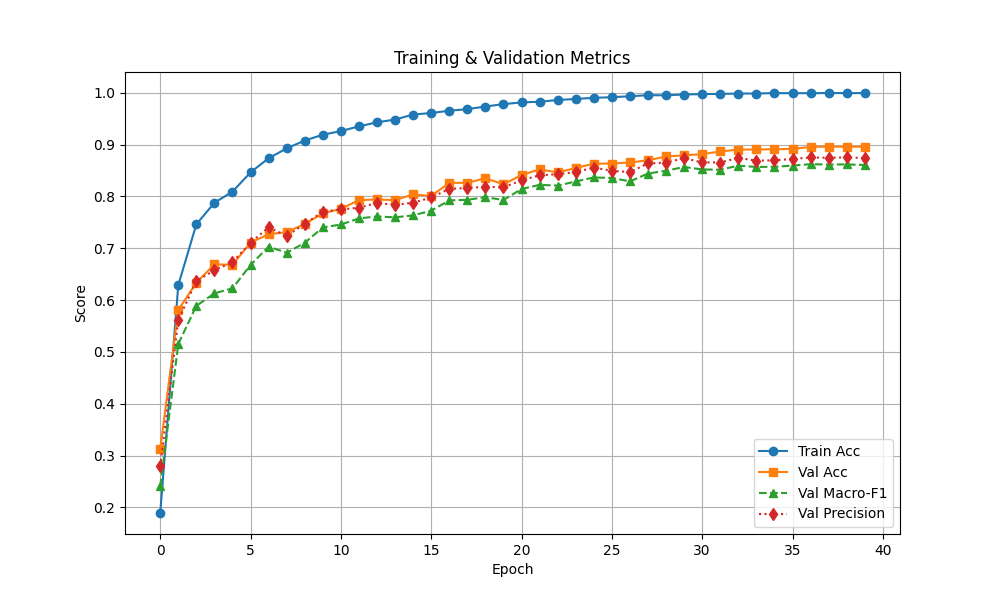
\includegraphics[width=\linewidth]{experiment_assets/training_curves/vit_b16_metrics.png}
        \caption{Training metrics for the ViT-B/16 model.} \label{fig:vit_b16_metrics}
    \end{minipage}\hfill
    \begin{minipage}{0.24\linewidth}
        \centering
        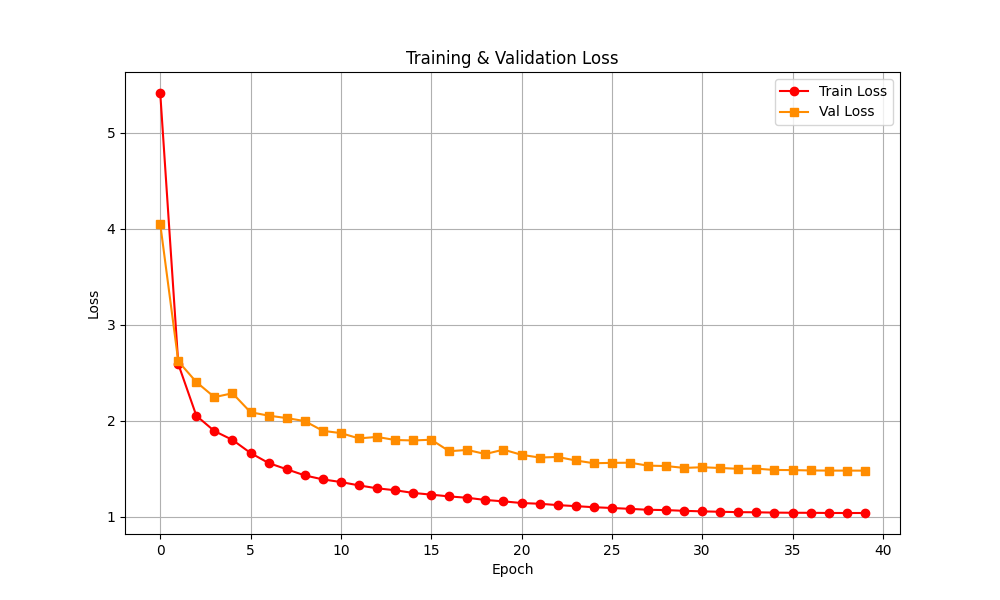
\includegraphics[width=\linewidth]{experiment_assets/training_curves/vit_b16_loss.png}
        \caption{Training loss for the ViT-B/16 model.} \label{fig:vit_b16_loss}
    \end{minipage}\hfill
    \begin{minipage}{0.24\linewidth}
        \centering
        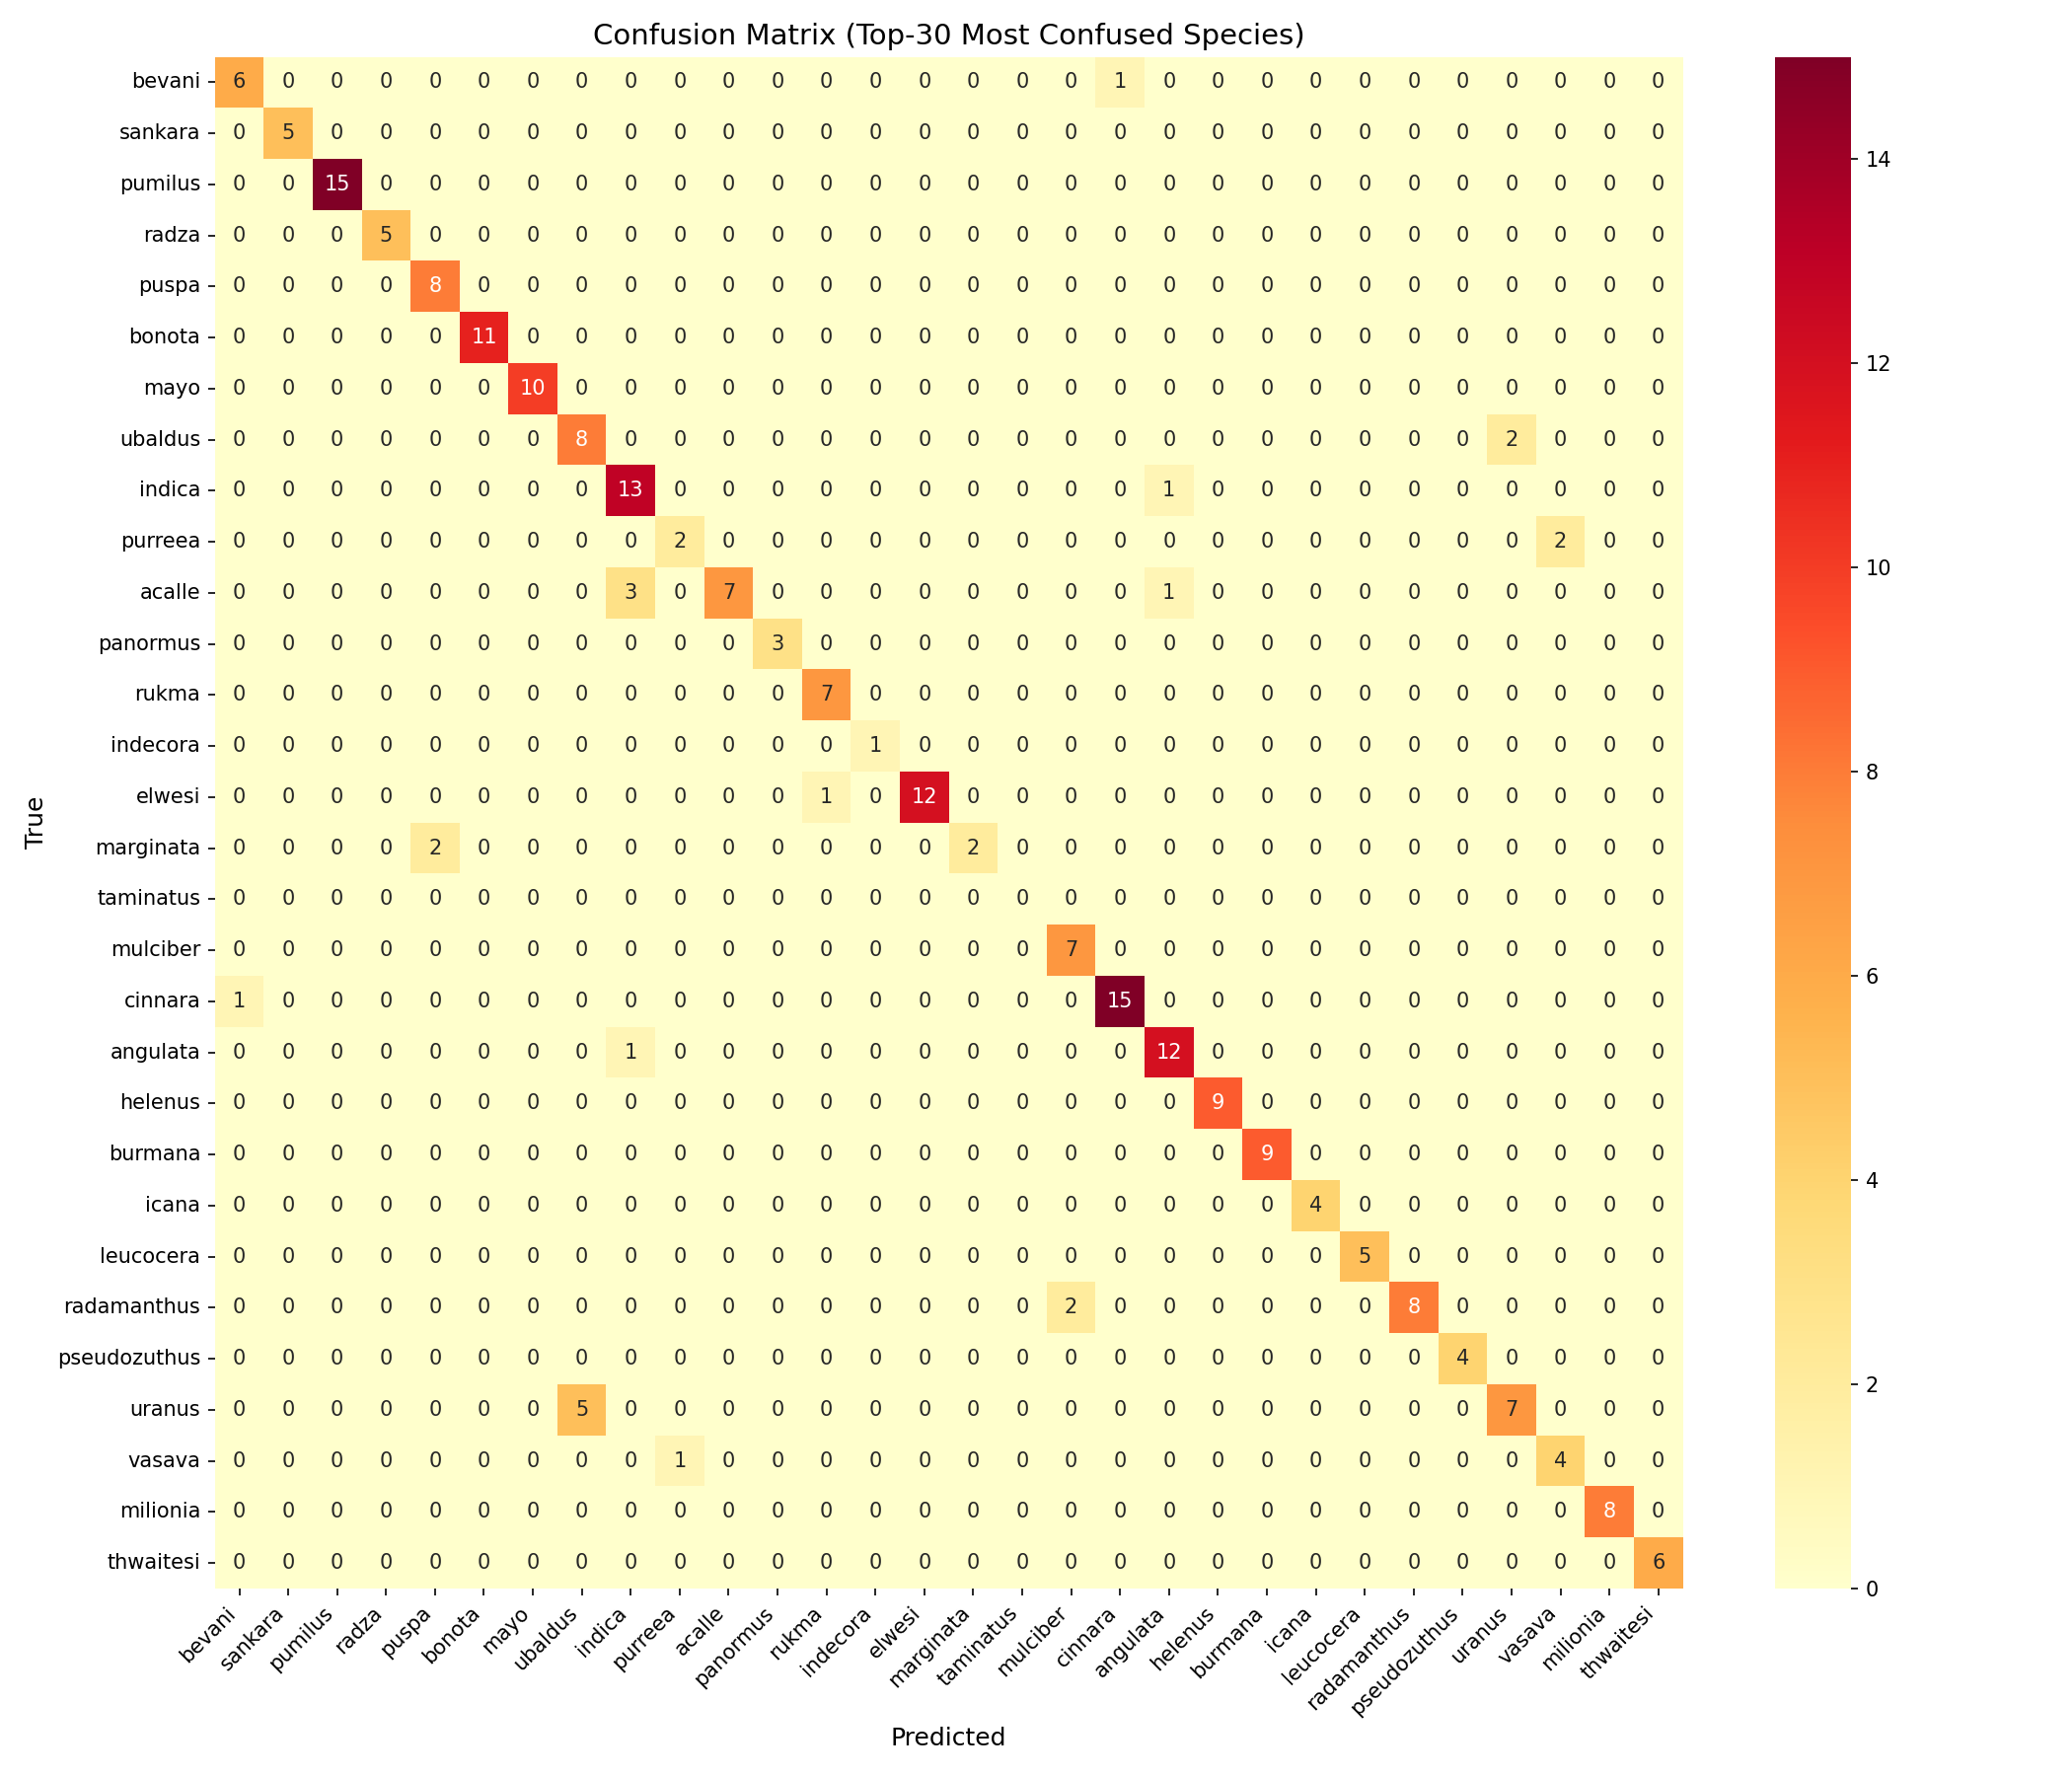
\includegraphics[width=\linewidth]{experiment_assets/confusion_matrices/vit_b16_confusion.png}
        \caption{Confusion matrix for ViT-B/16.} \label{fig:vit_b16_confusion}
    \end{minipage}\hfill
    \begin{minipage}{0.24\linewidth}\centering
        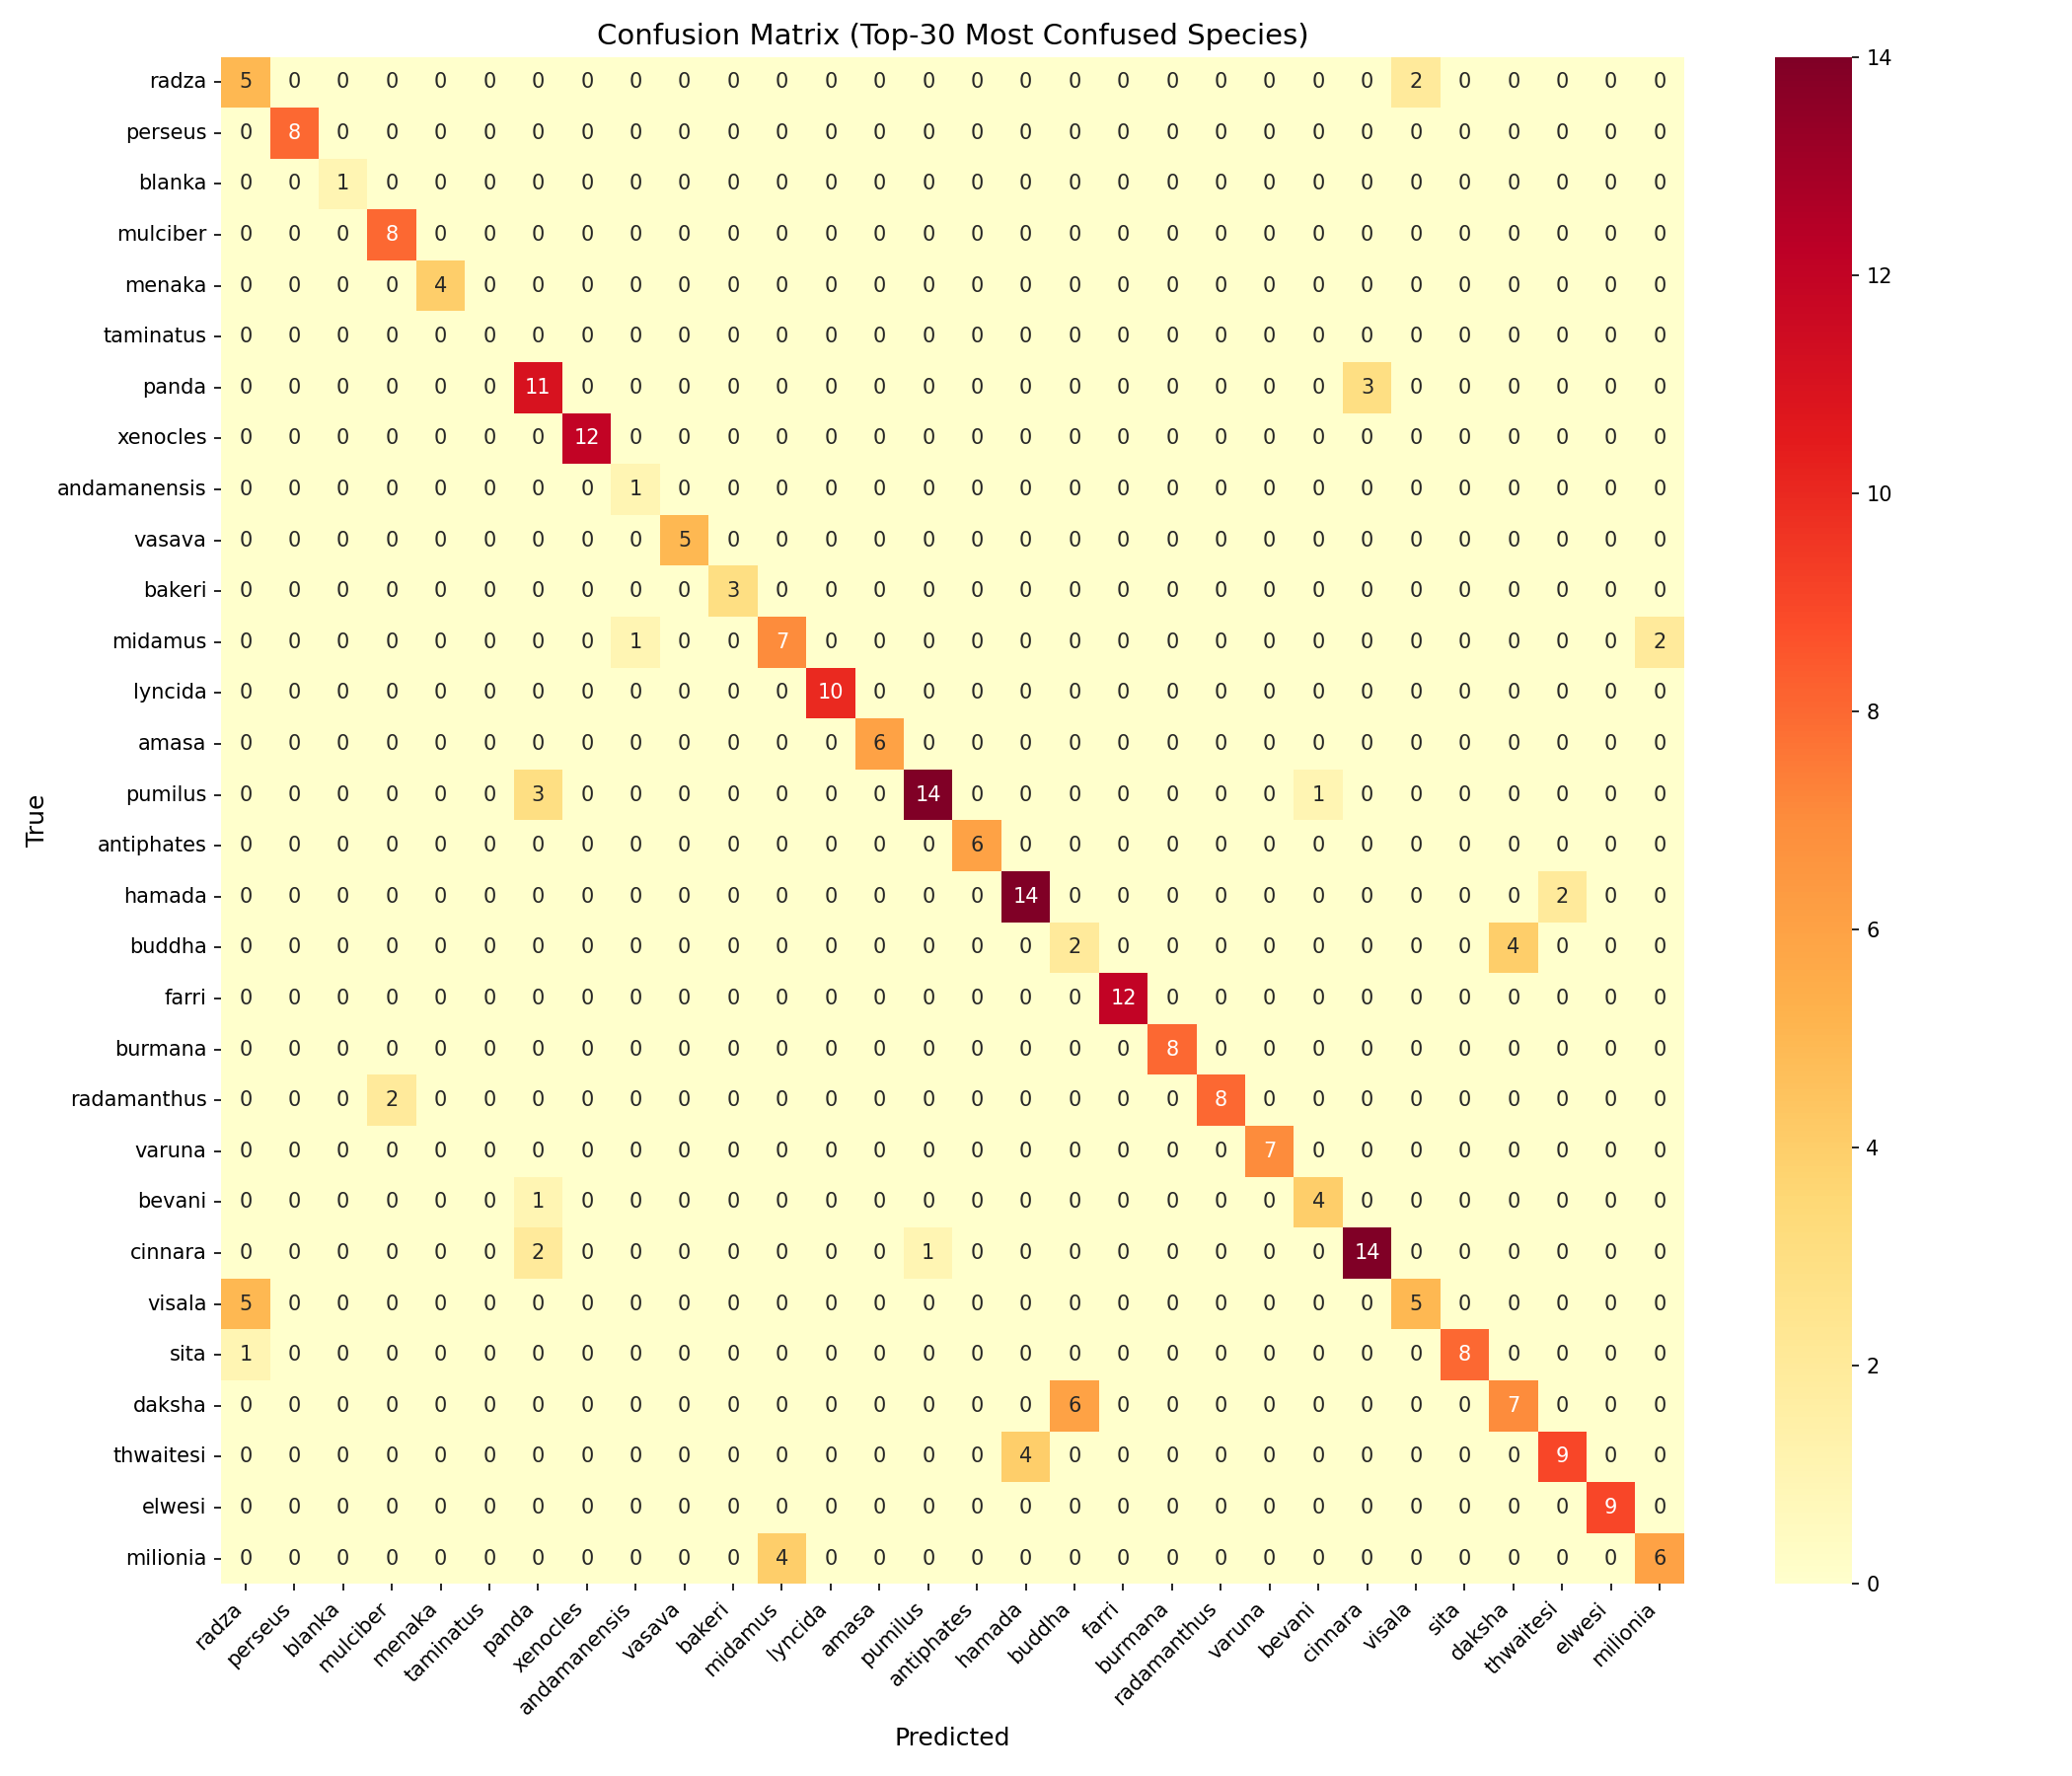
\includegraphics[width=\linewidth]{experiment_assets/confusion_matrices/geotemporal_confusion.png}
        \caption{Confusion matrix for Geotemporal.} \label{fig:geotemporal_confusion}
    \end{minipage}
\end{figure}
\vspace{0.2em}
\begin{figure}
    \centering
    \begin{minipage}{0.24\linewidth}
        \centering
        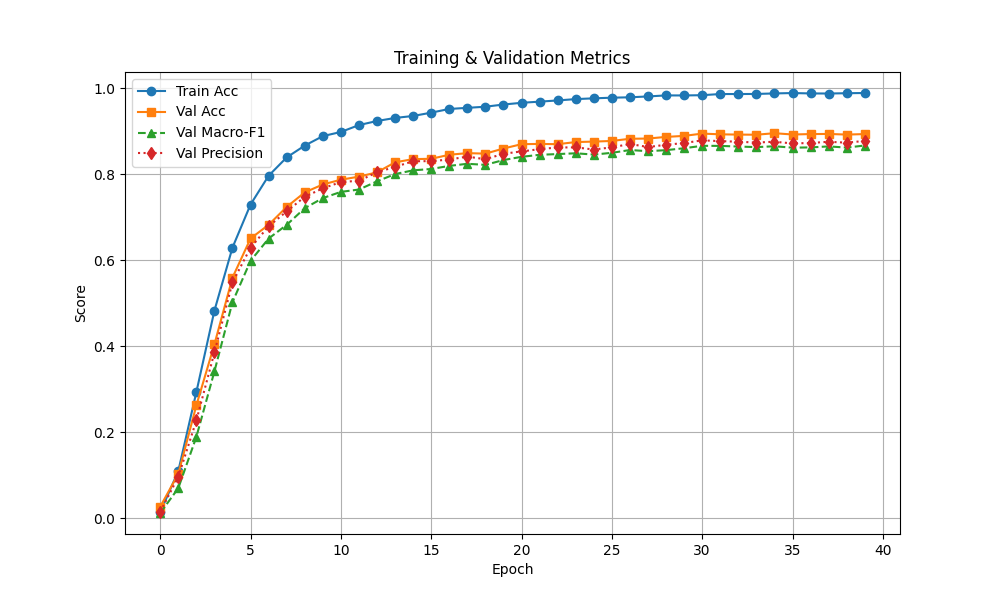
\includegraphics[width=\linewidth]{experiment_assets/training_curves/geotemporal_metrics.png}
        \caption{Training metrics for the Geotemporal model.} \label{fig:geotemporal_metrics}
    \end{minipage}\hfill
    \begin{minipage}{0.24\linewidth}
        \centering
        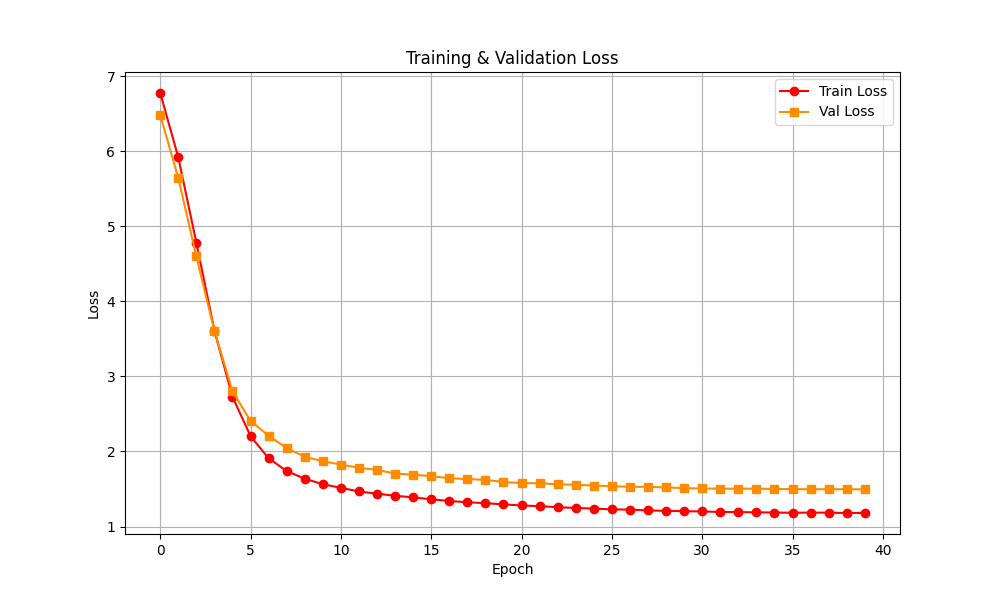
\includegraphics[width=\linewidth]{experiment_assets/training_curves/geotemporal_loss.png}
        \caption{Training loss for the Geotemporal model.} \label{fig:geotemporal_loss}
    \end{minipage}\hfill
    \begin{minipage}{0.24\linewidth}
        \centering
        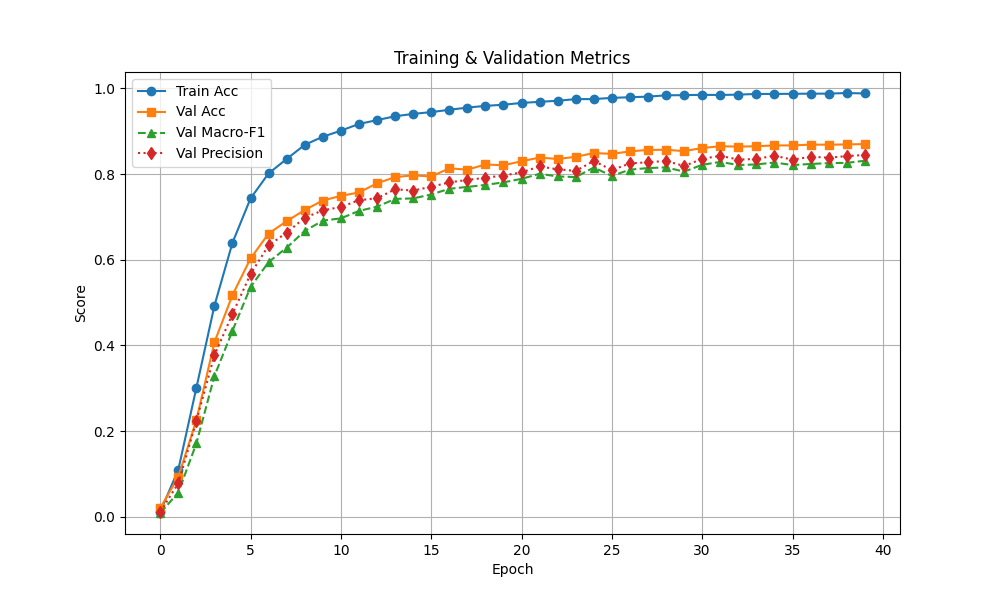
\includegraphics[width=\linewidth]{experiment_assets/training_curves/geo_shuffled_metrics.png}
        \caption{Training metrics for the Geo-Shuffled model.} \label{fig:geo_shuffled_metrics}
    \end{minipage}\hfill
    \begin{minipage}{0.24\linewidth}
        \centering
        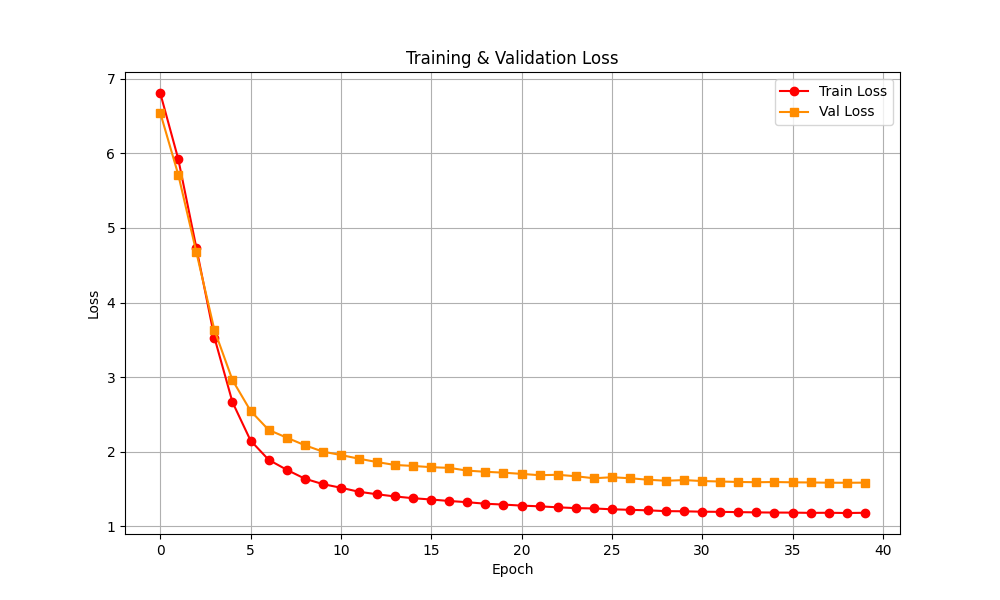
\includegraphics[width=\linewidth]{experiment_assets/training_curves/geo_shuffled_loss.png}
        \caption{Training loss for the Geo-Shuffled model.} \label{fig:geo_shuffled_loss}
    \end{minipage}
\end{figure}


\begin{figure}
    \centering
    \begin{minipage}{0.24\linewidth}\centering
        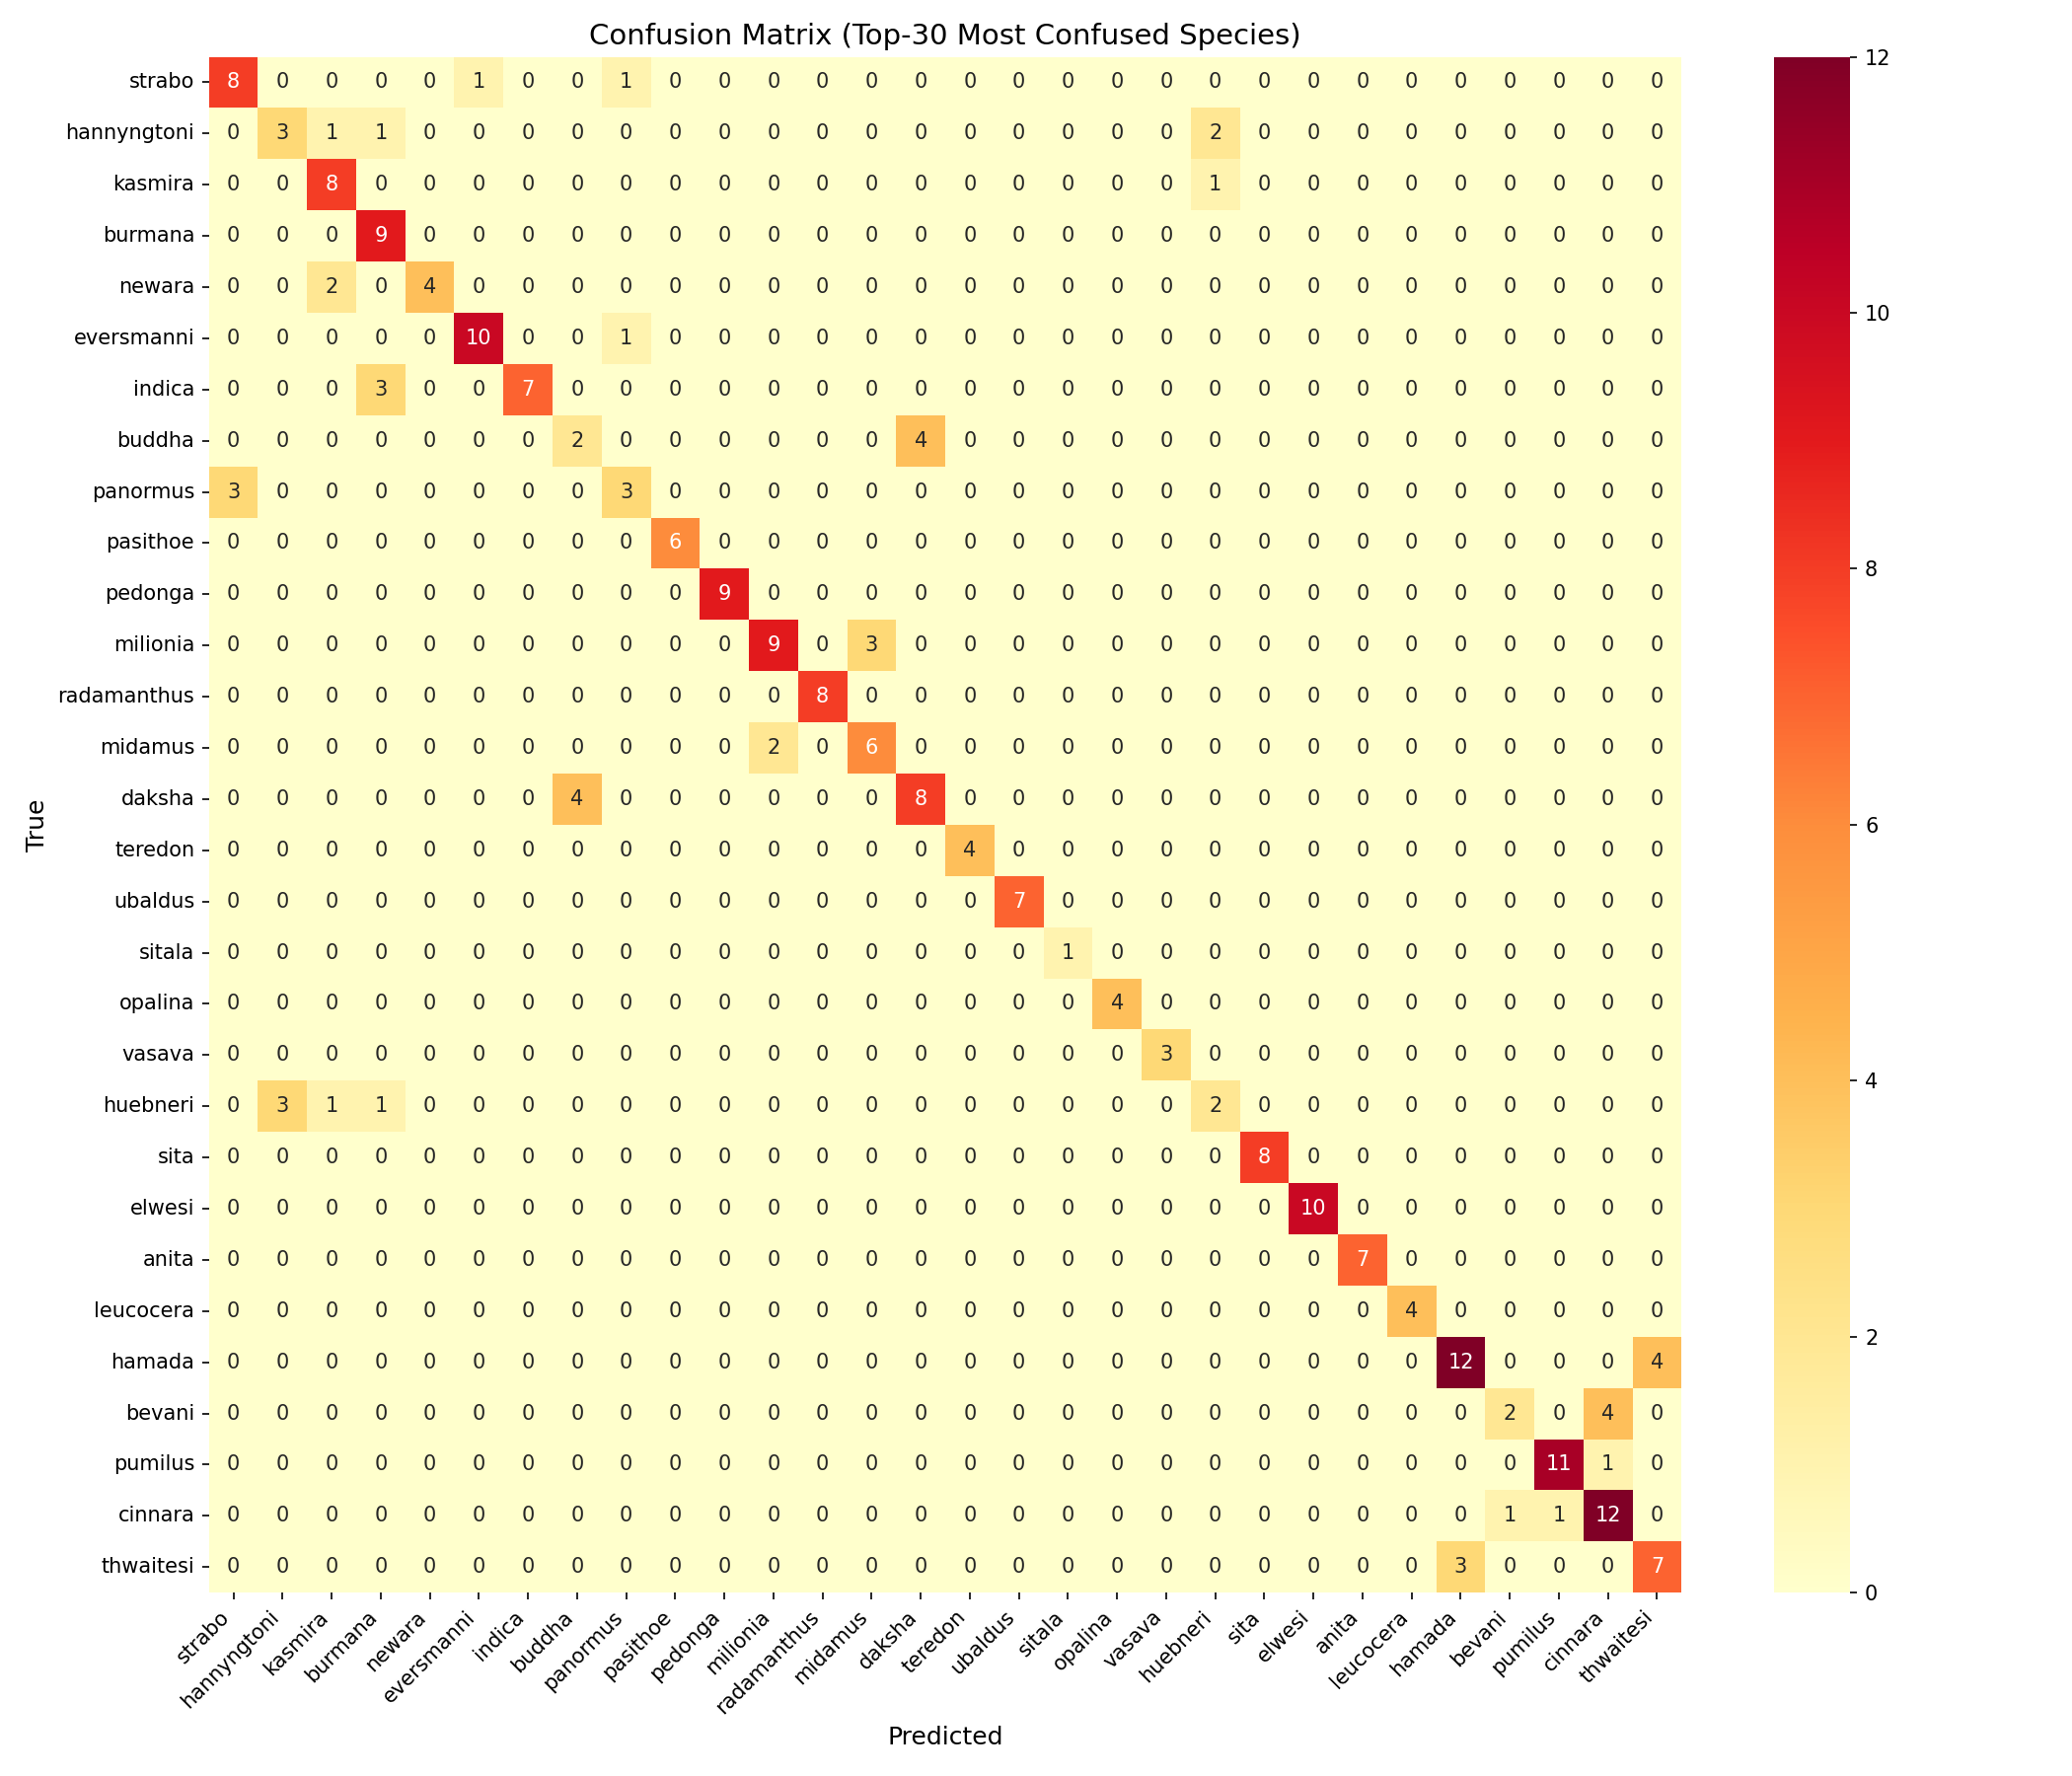
\includegraphics[width=\linewidth]{experiment_assets/confusion_matrices/geo_shuffled_confusion.png}
        \caption{Confusion matrix for Geo-Shuffled.} \label{fig:geo_shuffled_confusion}
    \end{minipage}\hfill
    \begin{minipage}{0.24\linewidth}\centering
        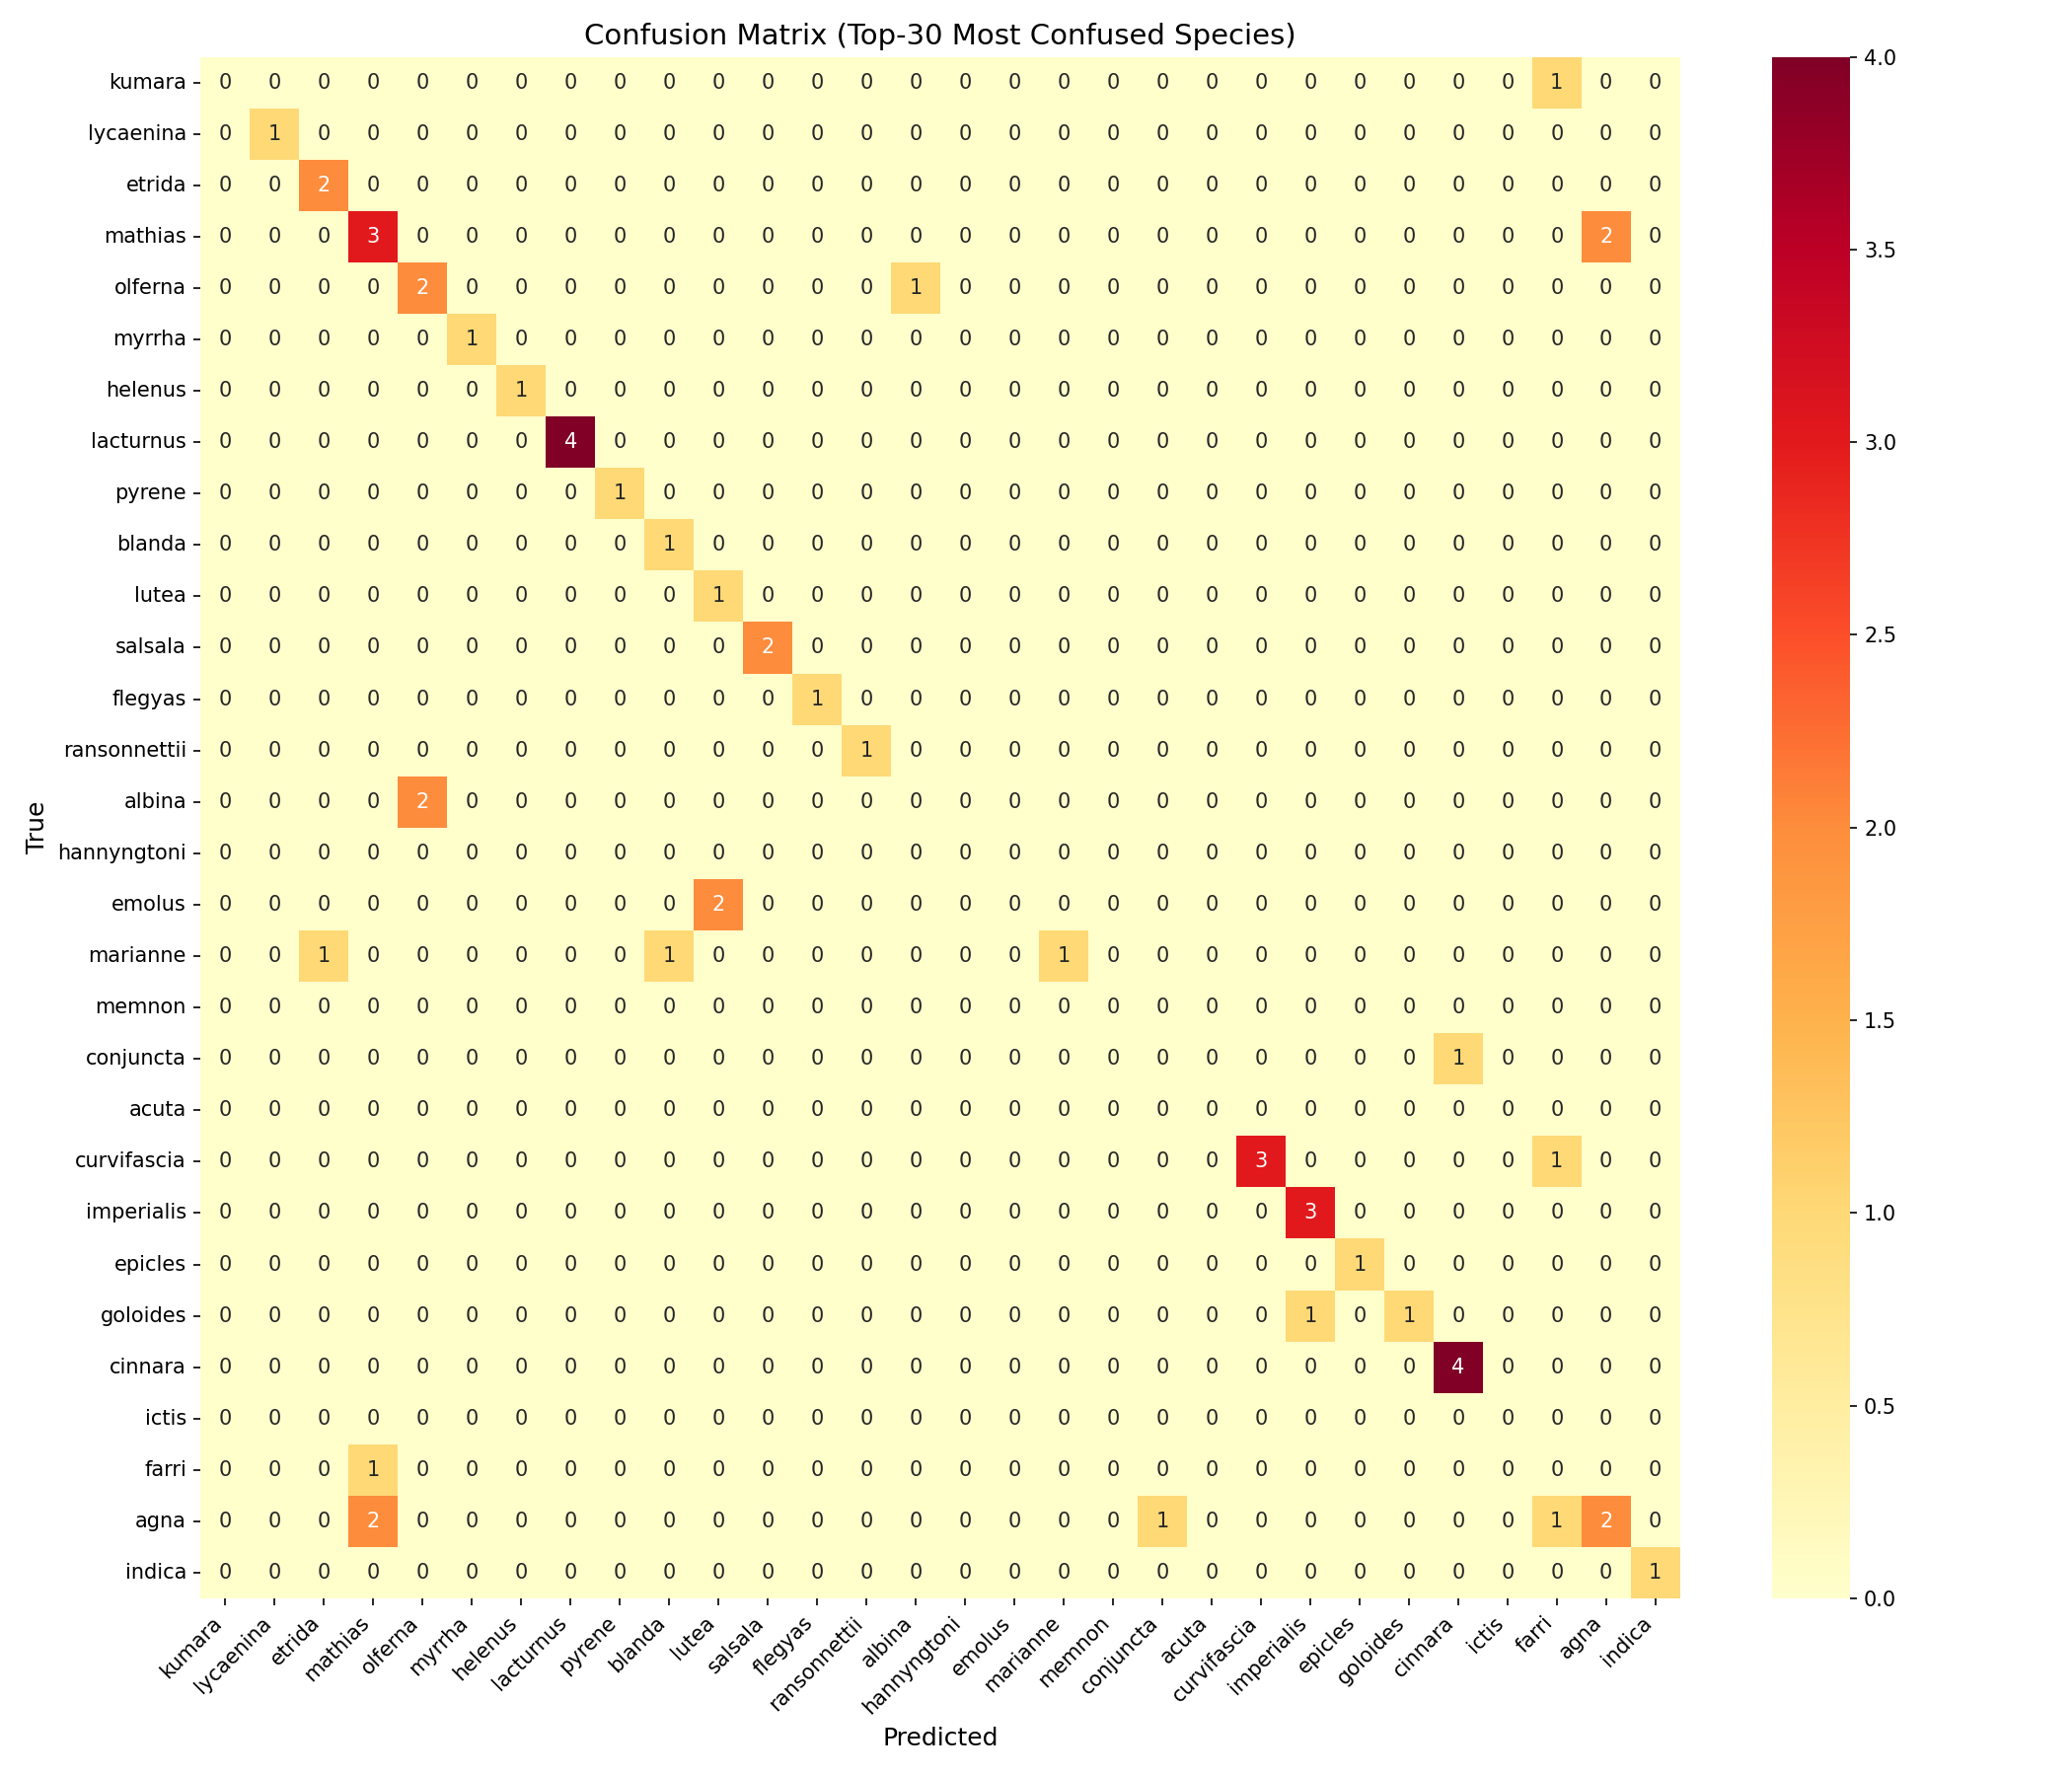
\includegraphics[width=\linewidth]{experiment_assets/confusion_matrices/resnet101_confusion.png}
        \caption{Confusion matrix for ResNet-101.} \label{fig:resnet101_confusion}
    \end{minipage}\hfill
    \begin{minipage}{0.24\linewidth}
        \centering
        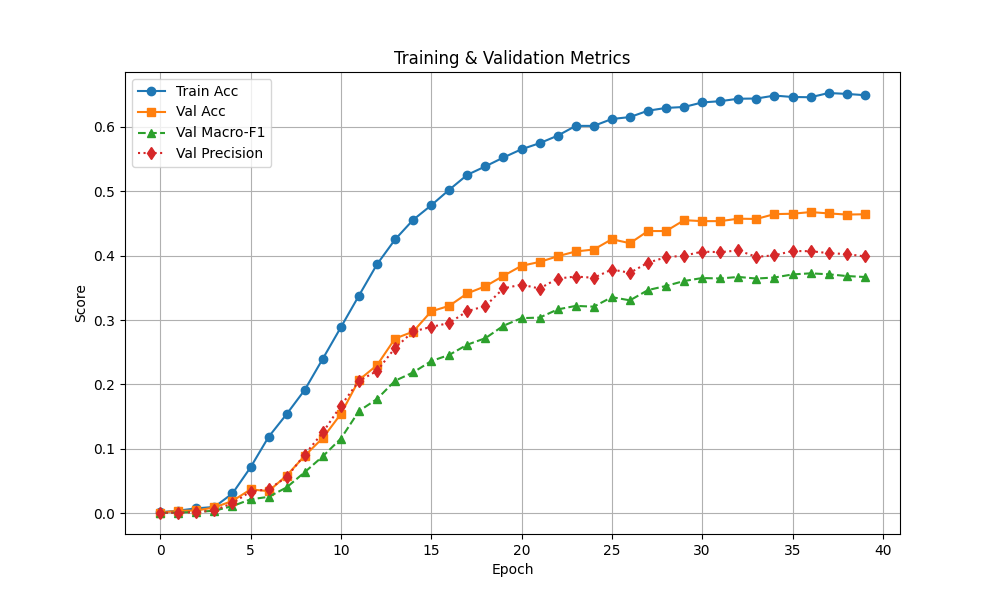
\includegraphics[width=\linewidth]{experiment_assets/training_curves/resnet101_metrics.png}
        \caption{Training metrics for the ResNet-101 model.} \label{fig:resnet101_metrics}
    \end{minipage}\hfill
    \begin{minipage}{0.24\linewidth}
        \centering
        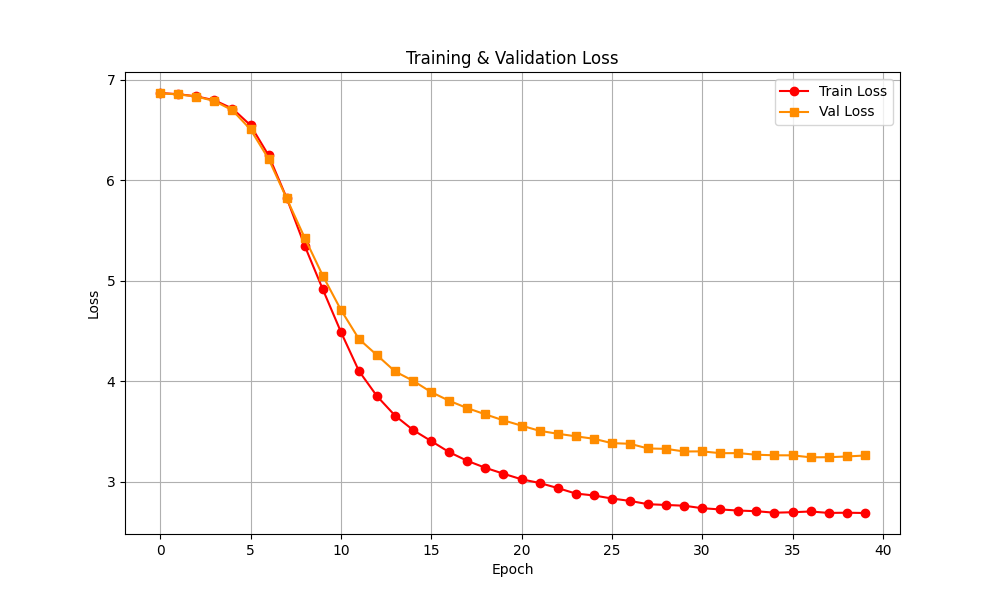
\includegraphics[width=\linewidth]{experiment_assets/training_curves/resnet101_loss.png}
        \caption{Training loss for the ResNet-101 model.} \label{fig:resnet101_loss}
    \end{minipage}
\end{figure}


\begin{figure}
    \centering
    \begin{minipage}{0.48\linewidth}
        \centering
        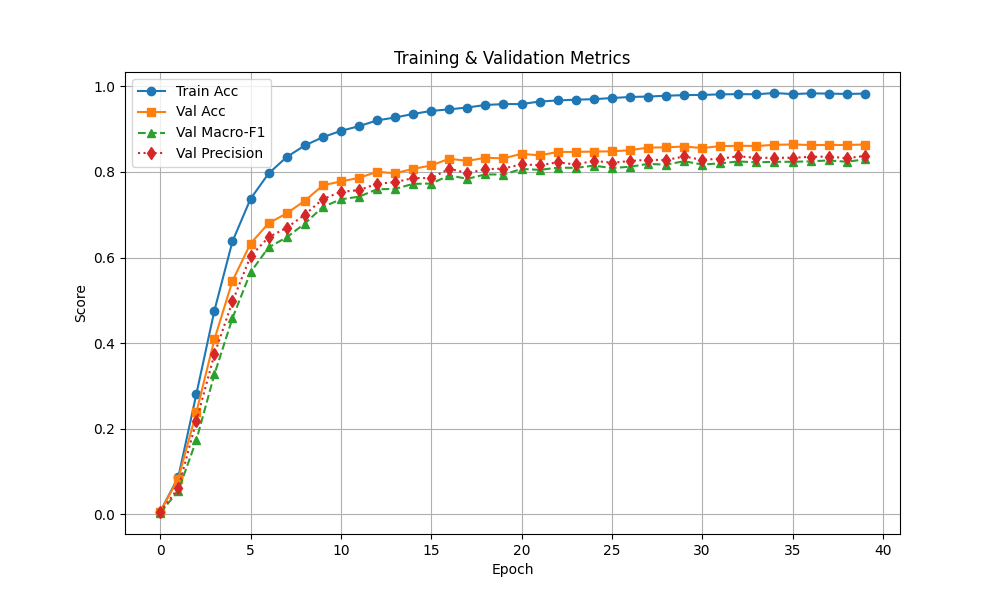
\includegraphics[width=\linewidth]{experiment_assets/training_curves/effnet_b5_metrics.png}
        \caption{Training metrics for the EfficientNet-B5 model.} \label{fig:effnet_b5_metrics}
    \end{minipage}\hfill
    \begin{minipage}{0.48\linewidth}
        \centering
        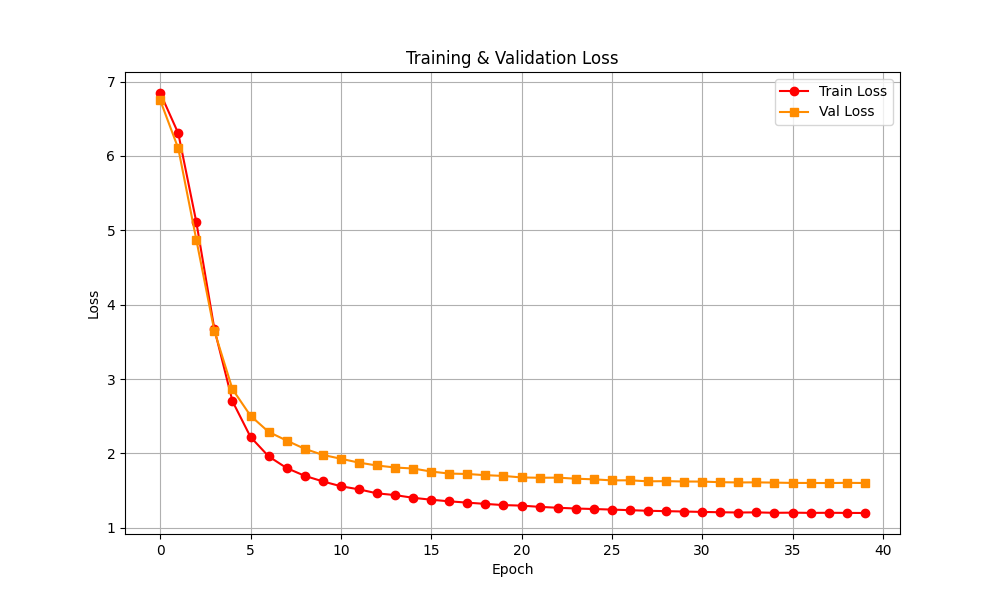
\includegraphics[width=\linewidth]{experiment_assets/training_curves/effnet_b5_loss.png}
        \caption{Training loss for the EfficientNet-B5 model.} \label{fig:effnet_b5_loss}
    \end{minipage}
\end{figure}

\begin{figure}
    \centering
    \begin{minipage}{0.24\linewidth}
        \centering
        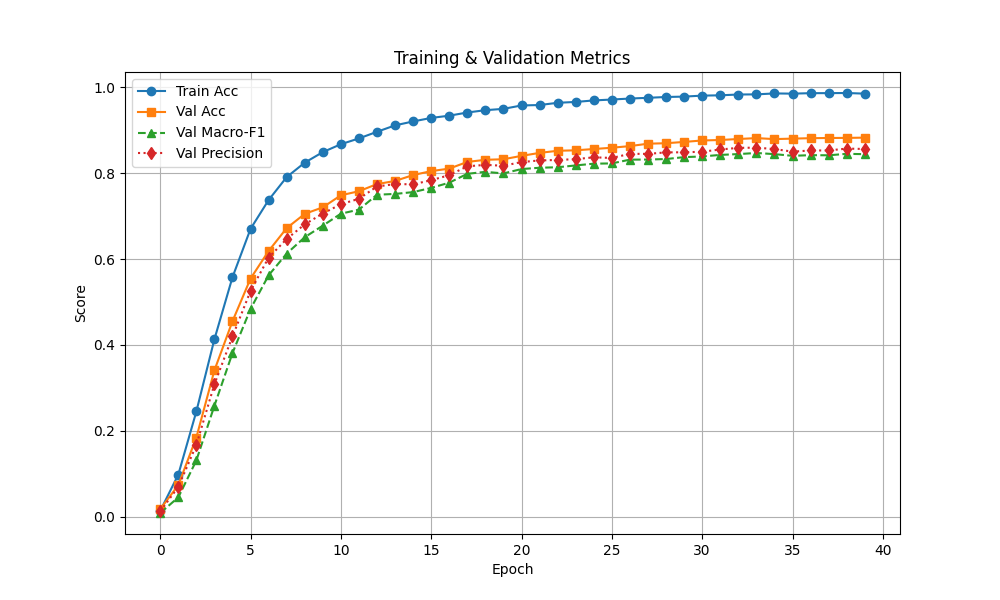
\includegraphics[width=\linewidth]{experiment_assets/training_curves/mlfi_warmup_metrics.png}
        \caption{Training metrics for the MLFI Warmup model.} \label{fig:mlfi_warmup_metrics}
    \end{minipage}\hfill
    \begin{minipage}{0.24\linewidth}
        \centering
        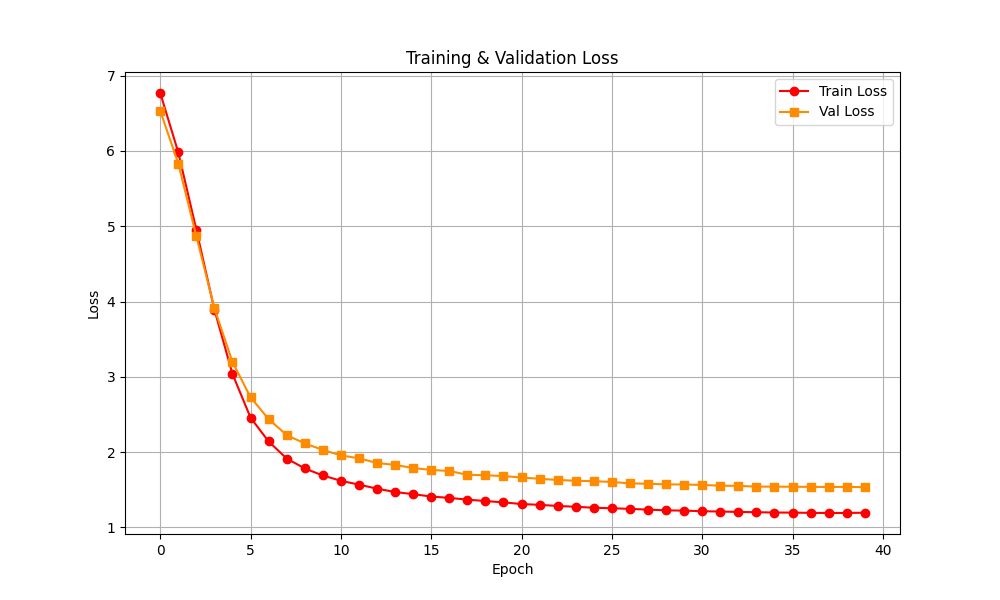
\includegraphics[width=\linewidth]{experiment_assets/training_curves/mlfi_warmup_loss.png}
        \caption{Training loss for the MLFI Warmup model.} \label{fig:mlfi_warmup_loss}
    \end{minipage}\hfill
    \begin{minipage}{0.24\linewidth}\centering
        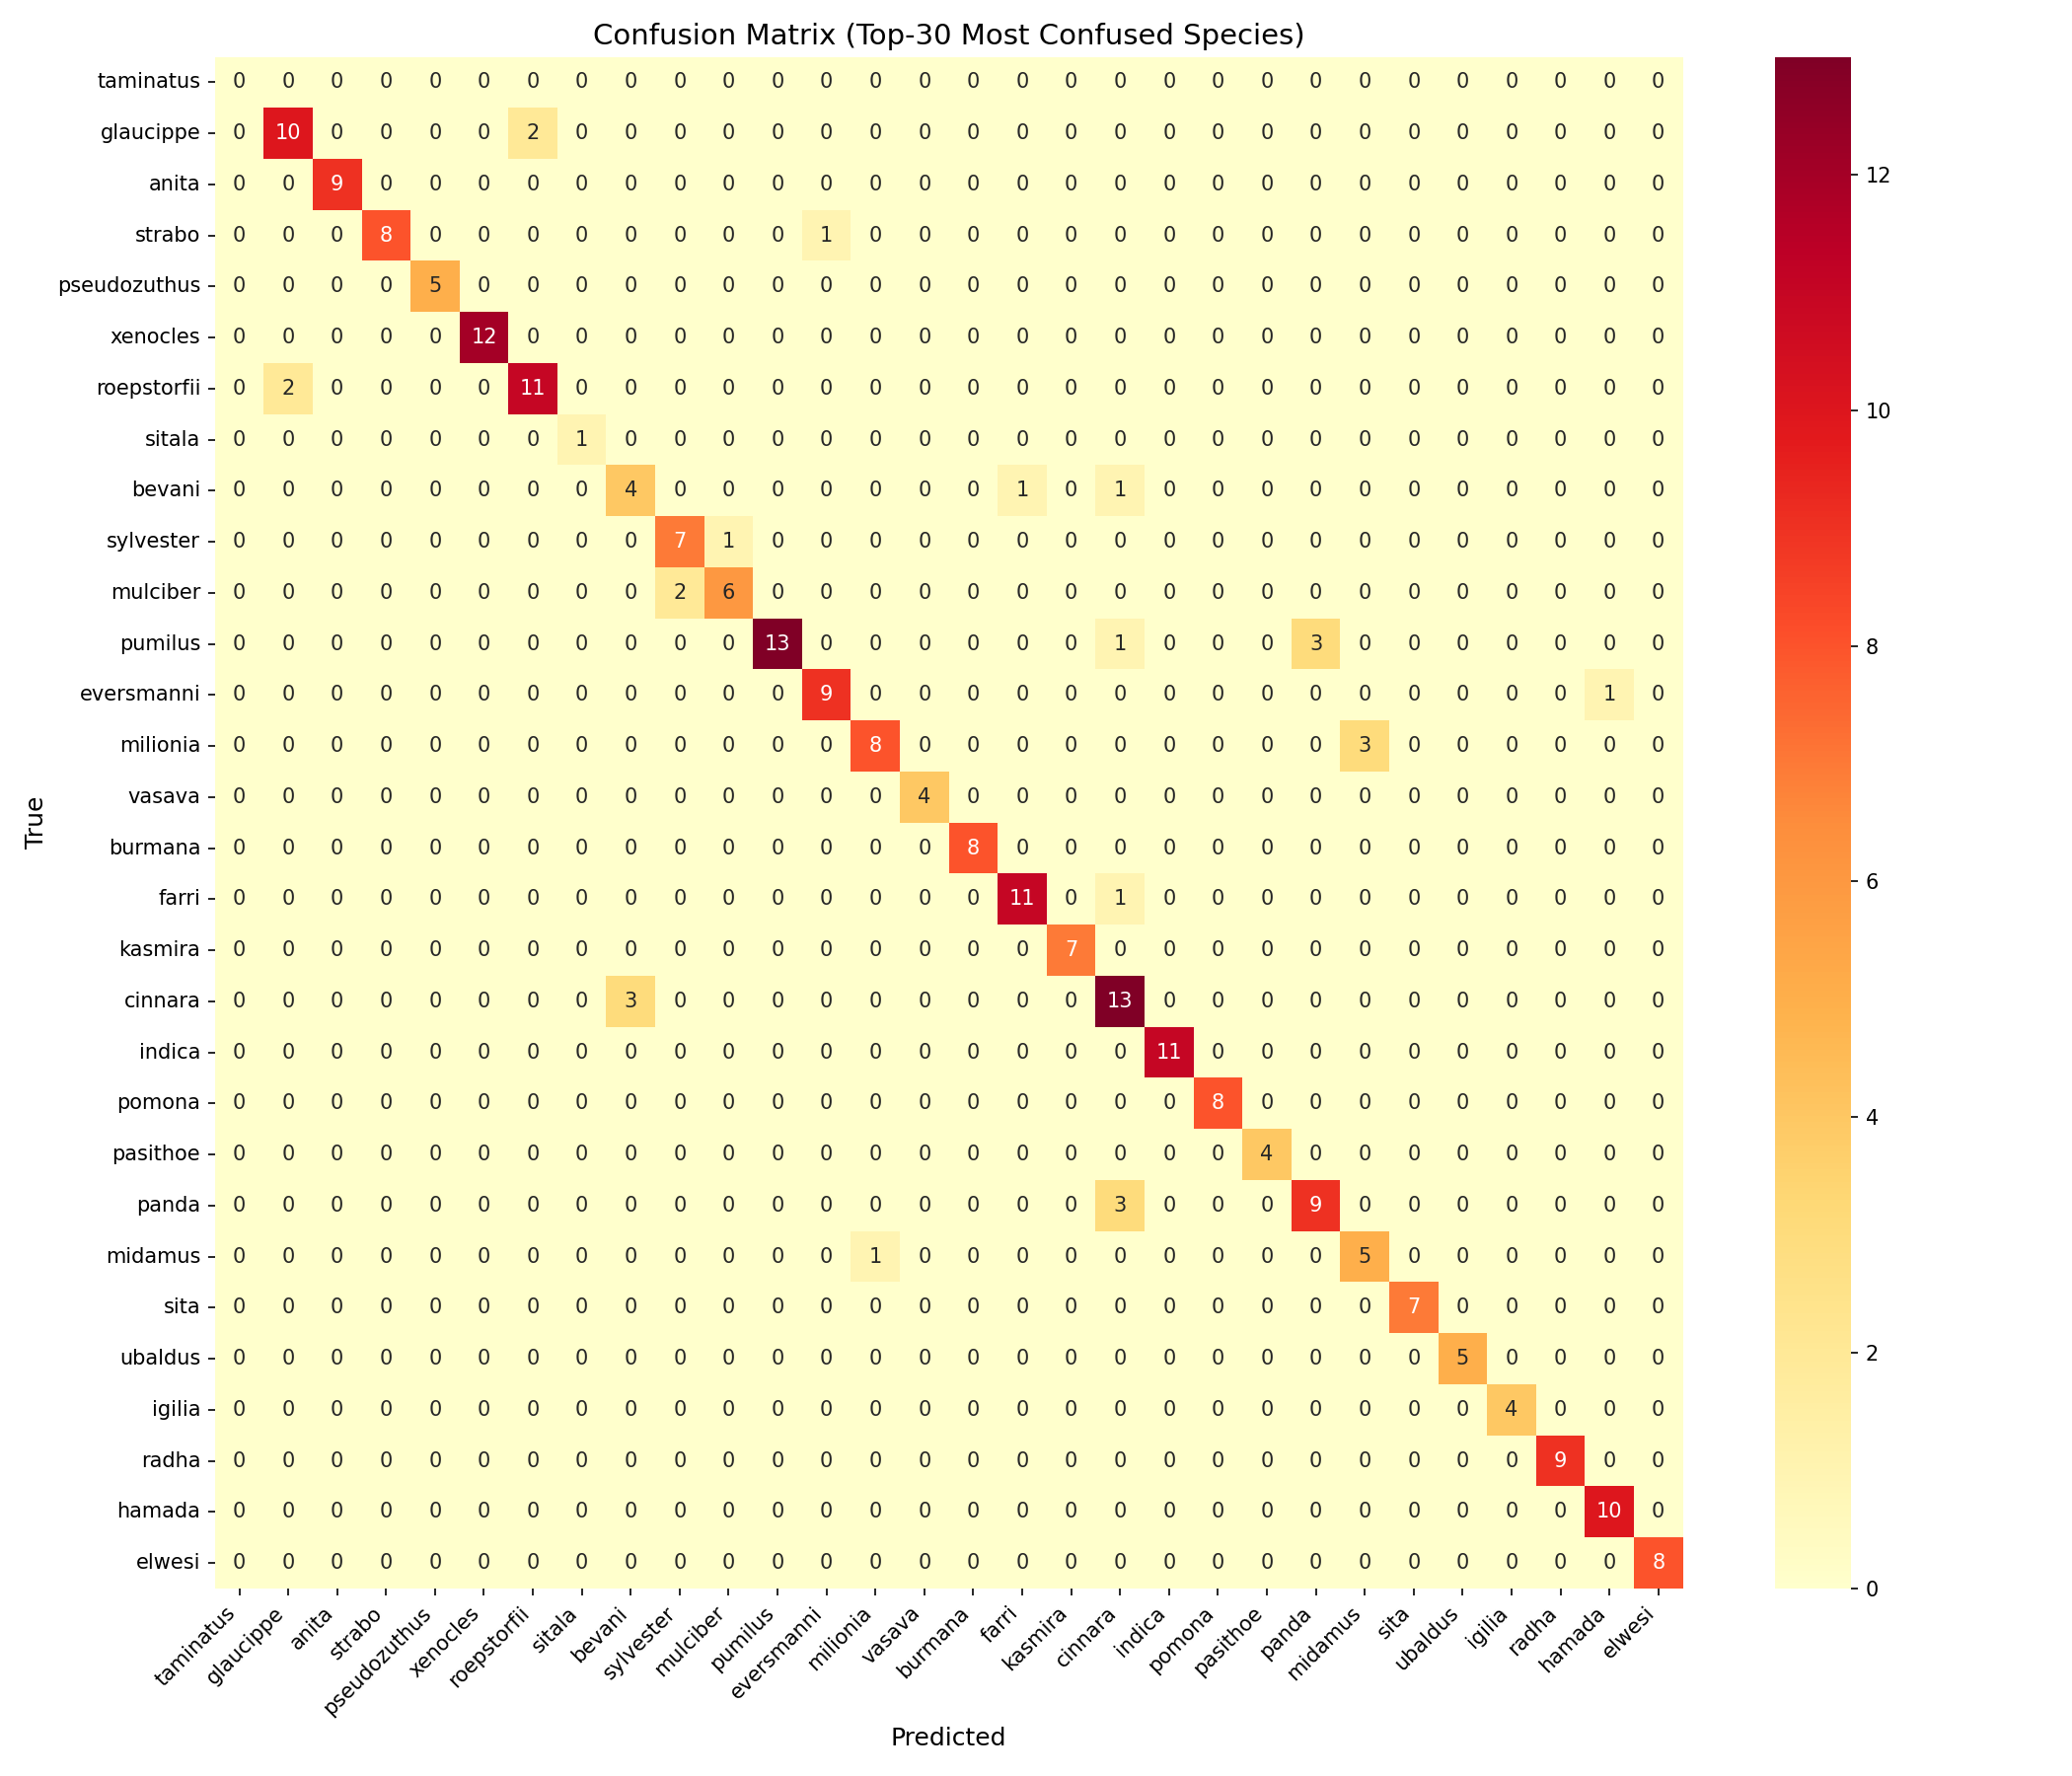
\includegraphics[width=\linewidth]{experiment_assets/confusion_matrices/effnet_b5_confusion.png}
        \caption{Confusion matrix for EfficientNet-B5.} \label{fig:effnet_b5_confusion}
    \end{minipage}\hfill
    \begin{minipage}{0.24\linewidth}\centering
        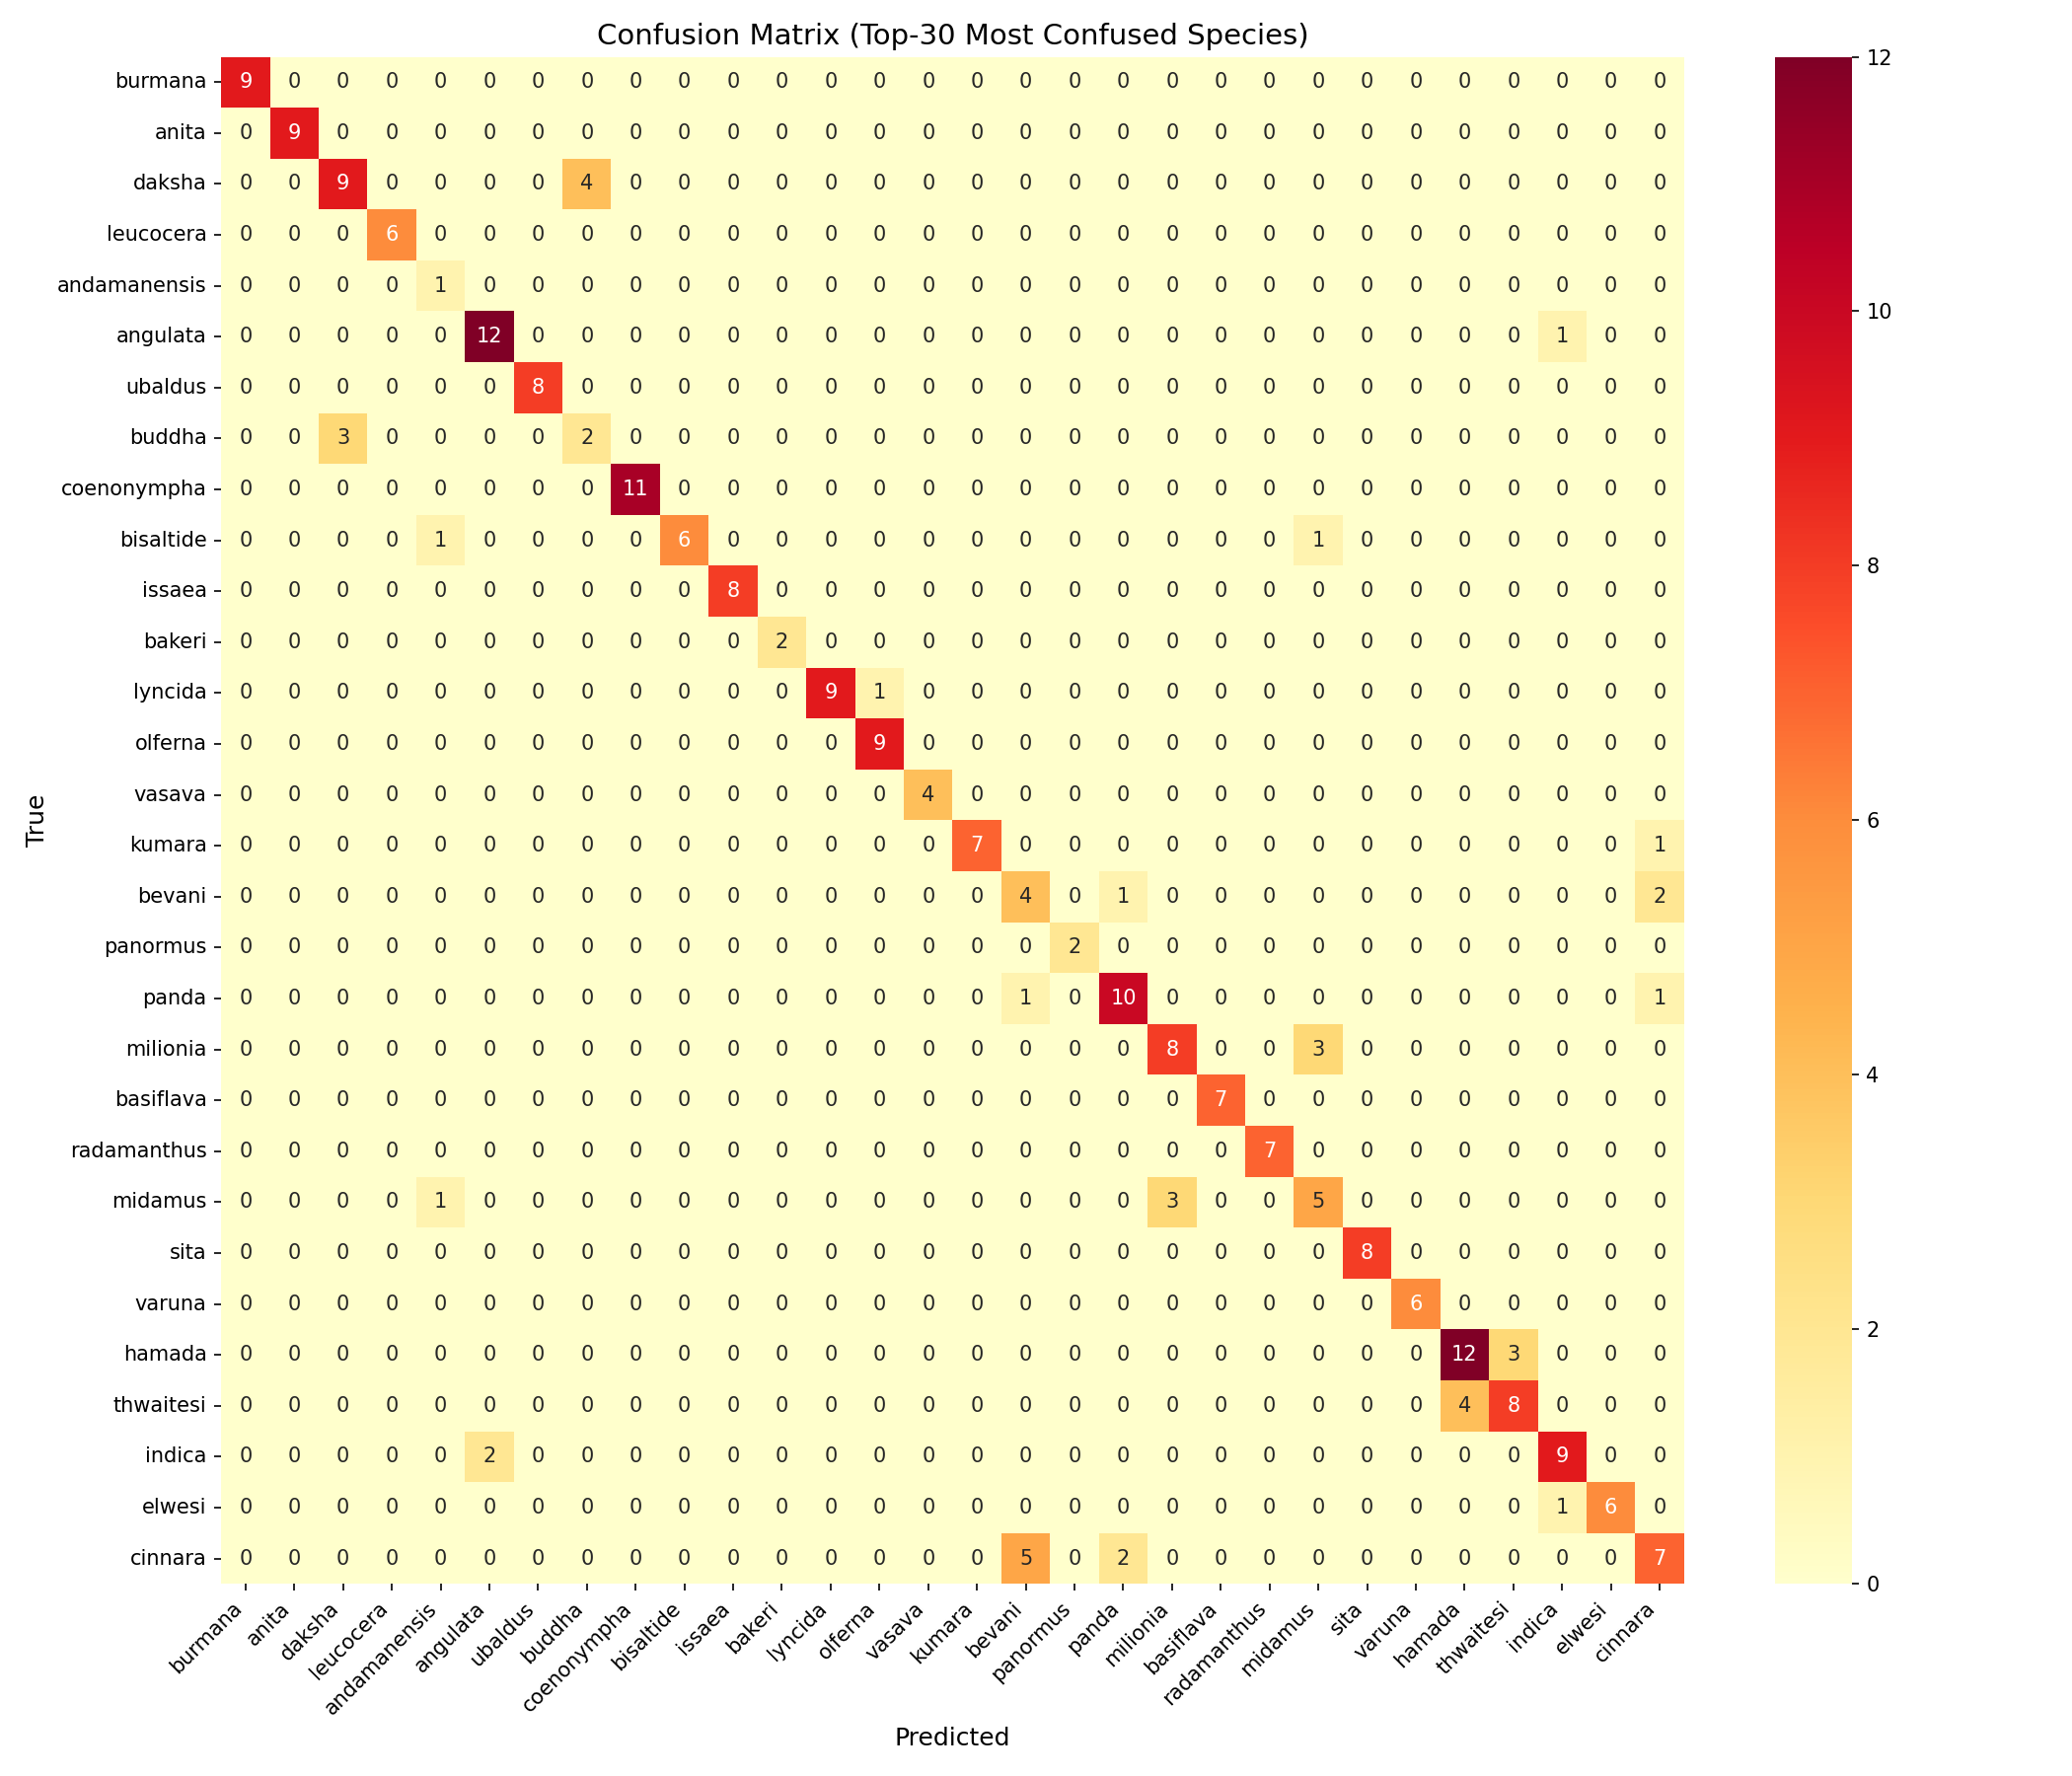
\includegraphics[width=\linewidth]{experiment_assets/confusion_matrices/mlfi_warmup_confusion.png}
        \caption{Confusion matrix for MLFI Warmup.} \label{fig:mlfi_warmup_confusion}
    \end{minipage}
\end{figure}


\subsection{Per-Stratum Analysis}
\begin{table}[H]
    \centering
    \caption{Per-Stratum Analysis}
    \begin{tabular}{|l|l|l|l|l|l|}
        \toprule
        \textbf{Model} & \textbf{Dense Acc (\%)} & \textbf{Dense F1 (\%)} & \textbf{Sparse Acc (\%)} & \textbf{Sparse F1 (\%)} & \textbf{$\Delta$ Acc ($\text{Sp}_{Dense}$)} \\
        \midrule
        ResNet-101 & 45.02\% & 22.53\% & 56.29\% & 45.80\% & +11.27\\
        EfficientNet-B5 & 87.33\% & 68.30\% & 86.20\% & 75.07\% & -1.13\\
        ViT-B/16 & \textbf{91.60\%} & \textbf{79.40\%} & 86.76\% & 75.18\% & -4.84\\
        MLFI Warmup & 88.36\% & 73.07\% & 84.86\% & 72.84\% & -3.50\\
        Geo-Shuffled & 87.87\% & 72.32\% & 83.32\% & 71.89\% & -4.55\\
        \textbf{Geotemporal (Ours)} & 90.35\% & 76.74\% & \textbf{87.43\%} & \textbf{75.38\%} & -2.92\\
        \bottomrule
    \end{tabular}
    \label{tab:per_stratum_analysis}
\end{table}

\subsection{Confusion Matrix Analysis}
\begin{table}[H]
    \centering
    \caption{Confusion Matrix Analysis}
    \begin{tabular}{|l|l|l|l|}
        \toprule
        \textbf{Model} & \textbf{True Species} & \textbf{Predicted As} & \textbf{Count} \\
        \midrule
 ResNet-101 & \textit{Symbrenthia brabira} & \textit{S. lilaea} & 7 \\
 ResNet-101 & \textit{Eurema blanda} & \textit{E. hecabe} & 7 \\
 EfficientNet-B5 & \textit{Azanus ubaldus} & \textit{A. uranus} & 6 \\
 EfficientNet-B5 & \textit{Tarucus indica} & \textit{T. nara} & 5 \\
 ViT-B/16 & \textit{Tapena thwaitesi} & \textit{Taraka hamada} & 8 \\
 ViT-B/16 & \textit{Azanus uranus} & \textit{A. ubaldus} & 5 \\
 Geotemporal & \textit{Papilio daksha} & \textit{P. buddha} & 6 \\
 Geotemporal & \textit{Mycalesis visala} & \textit{M. radza} & 5 \\
        \bottomrule
    \end{tabular}
    \label{tab:confusion_matrix_analysis}
\end{table}

\subsection{Key Findings}
\begin{enumerate}
    \item \textbf{Geotemporal fusion} is competitive with \textbf{ViT-B/16.} Achieves 89.38\% Top-1 with \textit{2.1$\times$ fewer parameters}. It achieves the \textbf{best Top-5 accuracy (98.01\%)} across all models.
    \item \textbf{Geotemporal metadata provides a genuine signal.} The geo-shuffled control (same architecture, randomised location/month) drops by: $-3.02\%$ Top-1 (89.38 $\to$ 86.36) and $-2.80\%$ Macro F1 (87.37 $\to$ 84.57). The geotemporal branch learns meaningful biogeographic priors, does not just adds parameters.
    \item \textbf{Best sparse-class performance from geotemporal model.} 87.43\% accuracy on sparse classes (<50 training images), outperforming all baselines including ViT-B/16 (86.76\%). The Dense–Sparse gap narrows to $\Delta$ = $-2.92$ vs ViT-B/16's $\Delta$ = $-4.84$, suggesting geotemporal priors help disambiguate underrepresented species.
    \item \textbf{MLFI warmup provides modest gains.} 87.20\% vs 86.36\% (geo-shuffled), but underperforms full geotemporal fusion (89.38\%), suggesting multi-level feature integration benefits from geospatial context.
\end{enumerate}

\section{Discussion}

Our study highlights why architectural design and ecological and temporal context are critical for fine-grained biological classification. Three structural constraints drive the primary failure modes:

\begin{itemize}
    \item \textbf{Spatial Collapse} Coordinate Attention addresses spatial collapse by preserving the directional structure of butterfly morphology (e.g., horizontal bands vs. vertical veins). Adding CA requires $<$0.5\% more parameters but improves sparse-class accuracy by 1.29 points.

    \item \textbf{Texture Loss} MLFI preserves essential early-layer texture features, but requires careful optimisation. Applying a learning rate warmup to newly initialised branches recovers a \textbf{2.77-point Top-1 improvement} over the unwarmed baseline (87.20\% vs. 84.43\%).

    \item \textbf{Domain Shift} The failure of Head-Only fine-tuning (53.20\%) highlights a severe domain shift from natural images to biological specimens. ImageNet features encode object silhouettes rather than critical fine-grained features like submarginal bands, making full end-to-end recalibration essential for transferability.

    \item \textbf{Geotemporal Signal} Beyond architecture, geotemporal fusion bridges the remaining accuracy gap by encoding biological reality. The most visually confused species pairs (\textit{Kalilima Inachus} $\leftrightarrow$ \textit{Kalilima Horsfieldii}, \textit{Malabar Rose} $\leftrightarrow$ \textit{Common Rose}, \textit{Mycalesis Francisca} $\leftrightarrow$ \textit{Mycalesis Gotama}) are congeneric species with overlapping wing patterns but \textbf{distinct geographic ranges and flight seasons}, the additional context the geotemporal embeddings provide for disambiguiation.
\end{itemize}

\section{Conclusion}

IndoLepAtlas fills a documented gap in the insect classification literature as the first India-specific Lepidoptera dataset with integrated geotemporal metadata, early life-stage documentation, and host plant associations. By establishing a 60,641-image baseline covering 967 species, we aim to bridge a major gap in region--based ecological classification.

Our evaluations demonstrate that modern architectures require targeted adaptations for biological classification. Standard ImageNet transfer fails due to severe domain shifts, making end-to-end fine-tuning mandatory. However, combining Coordinate Attention with balanced sampling creates an efficient baseline that mitigates both spatial collapse and long-tail imbalance. Crucially, our geotemporal fusion module proves that integrating biogeographic and seasonal context provides genuine discriminative signal, bridging the accuracy gap to match much larger Vision Transformers at half the parameter cost.

\subsection{Future Work}
\begin{itemize}
    \item  \textbf{Prototypical network heads} for the ~533 classes with <50 images, enabling few-shot classification of rare species.
    \item  \textbf{Domain-specific self-supervised pretraining} (DINO/MAE on butterfly images) to bootstrap features from unlabelled in-domain data, reducing dependence on ImageNet initialisation.
    \item  \textbf{Host plant association features} for habitat-aware species prediction
    \item \textbf{Early stage detection} for conservation and finer species identification.
    \item  \textbf{Hierarchical classification} exploiting the taxonomic tree (family $\rightarrow$ genus $\rightarrow$ species) to reduce confusion between congeneric species.
\end{itemize}

\begin{credits}
\subsubsection{\ackname}
This work was carried out using the DGX V100 cluster at the LNM Institute of Information Technology. We thank the contributors of \href{https://www.ifoundbutterflies.org}{IFoundButterflies.org} for making the primary image data publicly available.

\subsubsection{\discintname}
The authors have no competing interests to declare that are relevant to the content of this article.
\end{credits}
%
% ---- Bibliography ----
%
% BibTeX users should specify bibliography style 'splncs04'.
% References will then be sorted and formatted in the correct style.
%
% \bibliographystyle{splncs04}
% \bibliography{mybibliography}
%
\begin{thebibliography}{16}

\bibitem{yuan2025fgbnet}
Yuan, Y. et~al.: FGBNet: A Bio-Subspecies Classification Network with Multi-Level Feature Interaction. \emph{Diversity} (2025). \url{https://doi.org/10.3390/d17040237}

\bibitem{hou2021coordinate}
Hou, Q., Zhou, D., Feng, J.: Coordinate Attention for Efficient Mobile Network Design. In: \emph{CVPR} (2021). \url{https://arxiv.org/abs/2103.02907}

\bibitem{liu2022convnext}
Liu, Z., Mao, H., Wu, C.-Y., Feichtenhofer, C., Darrell, T., Xie, S.: A ConvNet for the 2020s. In: \emph{CVPR} (2022). \url{https://arxiv.org/abs/2201.03545}

\bibitem{hu2018squeeze}
Hu, J., Shen, L., Sun, G.: Squeeze-and-Excitation Networks. In: \emph{CVPR} (2018). \url{https://arxiv.org/abs/1709.01507}

\bibitem{lin2017focal}
Lin, T.-Y., Goyal, P., Girshick, R., He, K., Doll\'{a}r, P.: Focal Loss for Dense Object Detection. In: \emph{ICCV} (2017). \url{https://arxiv.org/abs/1708.02002}

\bibitem{amarathunga2022thrips}
Amarathunga, D.C. et~al.: Fine-grained image classification of microscopic insect pest species. \emph{Computers and Electronics in Agriculture} (2022). \url{https://doi.org/10.1016/j.compag.2022.107462}

\bibitem{snell2017prototypical}
Snell, J., Swersky, K., Zemel, R.: Prototypical Networks for Few-Shot Learning. In: \emph{NeurIPS} (2017). \url{https://arxiv.org/abs/1703.05175}

\bibitem{feichtenhofer2022masked}
Feichtenhofer, C., Fan, H., Li, Y., He, K.: Masked autoencoders as spatiotemporal learners. In: \emph{NeurIPS} (2022)

\bibitem{dosovitski2021image}
Dosovitskiy, A. et~al.: An image is worth 16x16 words: Transformers for image recognition at scale. In: \emph{ICLR} (2021). \url{https://arxiv.org/abs/2010.11929}

\bibitem{loshchilov2017sgdr}
Loshchilov, I., Hutter, F.: SGDR: Stochastic Gradient Descent with Warm Restarts. In: \emph{ICLR} (2017). \url{https://arxiv.org/abs/1608.03983}

\bibitem{wah2011cub}
Wah, C., Branson, S., Welinder, P., Perona, P., Belongie, S.: The Caltech-UCSD Birds-200-2011 Dataset. Technical Report CNS-TR-2011-001, Caltech (2011)

\bibitem{vanhorn2018inaturalist}
Van~Horn, G. et~al.: The iNaturalist Species Classification and Detection Dataset. In: \emph{CVPR} (2018). \url{https://arxiv.org/abs/1707.06642}

\bibitem{amarathunga2021slr}
Amarathunga, D.C., Poskitt, J., Martini, A., Moreno-Garcia, J.: Methods of insect image capture and classification: a systematic literature review. \emph{Smart Agricultural Technology} \textbf{1}, 100023 (2021). \url{https://doi.org/10.1016/j.atech.2021.100023}

\bibitem{alfatemi2024birds}
Alfatemi, A., Abidin, Z.Z., Husin, Z., Abdul Aziz, K.A.: Multi-label classification with deep learning and manual data collection for identifying similar bird species. \emph{Computation} \textbf{12}(4), 77 (2024). \url{https://doi.org/10.3390/computation12040077}

\bibitem{wu2019ip102}
Wu, X., Zhan, C., Lai, Y.-K., Cheng, M.-M., Yang, J.: IP102: A large-scale benchmark dataset for insect pest recognition. In: \emph{CVPR}, pp.~8787--8796 (2019)

\bibitem{kehimkar2016butterflies}
Kehimkar, I.: Butterflies of India. Bombay Natural History Society, Mumbai (2016)

\end{thebibliography}

\end{document}
